
% Create well-known link to this spot for HTML version
\ifpdf
\else
\HCode{<a name='DUCC_INSTALL'></a>}
\fi
\chapter{Installation, Configuration, and Verification}
% 
% Licensed to the Apache Software Foundation (ASF) under one
% or more contributor license agreements.  See the NOTICE file
% distributed with this work for additional information
% regarding copyright ownership.  The ASF licenses this file
% to you under the Apache License, Version 2.0 (the
% "License"); you may not use this file except in compliance
% with the License.  You may obtain a copy of the License at
% 
%   http://www.apache.org/licenses/LICENSE-2.0
% 
% Unless required by applicable law or agreed to in writing,
% software distributed under the License is distributed on an
% "AS IS" BASIS, WITHOUT WARRANTIES OR CONDITIONS OF ANY
% KIND, either express or implied.  See the License for the
% specific language governing permissions and limitations
% under the License.
% 
\section{Overview}

DUCC is a multi-user, multi-system distributed application.  First-time installation is performed in
two stages:

\begin{itemize}
    \item Single-user installation: This provides single-user, single-system installation for testing,
      and verification. Simple development of small applications on small systems such as laptops or
      office workstations is possible after Single-user Installation.
      
    \item Multi-user installation: This provides secure multi-user capabilities and configuration
      for multi-system clusters.
\end{itemize}

First-time users must perform single-user installation and verification on a single system.  Once
this configuration is working and verified, it is straightforward to upgrade to a multi-user
configuration.

DUCC is distributed as a compressed tar file.  The instructions below assume installation from one
of this distribution media.  If building from source, the build creates this file in your svn
trunk/target directory. The distribution file is in the form
\begin{verbatim}
   apache-uima-ducc-[version].tar.gz
\end{verbatim}
where [version] is the DUCC version; for example, {\em \distro}.  This document will refer to the distribution
file as the ``$<$distribution.file$>$''.

\section{Software Prerequisites}
\label{sec:install.prerequisites}
Both single and multi-user configurations have the following software pre-requisites:

\begin{itemize}
  \item A userid {\em ducc}, and group {\em ducc}.  User {\em ducc} must the the only member of group {\em ducc}.
  \item Reasonably current Linux.  DUCC has been tested on SLES 10.2, 11.1, and 11.2, and RHEL 6.3.
    
    {\em Note:} On some systems the default {\em user limits}
    for max user processes (ulimit -u) and nfiles (ulimit -n) are defined too
    low for DUCC. The shell login profile for user {\em ducc} should set the
    soft limit for max user processes to be the same as the hard limit
    (ulimit -u `ulimit -Hu`), and
    the nfiles limit raised above 1024 to at least twice the number of user
    processes running on the cluster.

  \item For CGroupt support, libcgroup1-0.37+ on SLES and libcgroup-0.37+ on RHEL.  
  \item DUCC has been tested and run on IBM and Oracle JDK 1.6 and 1.7.
  \item Python 2.x, where 'x' is 4 or greater.  DUCC has not been tested on Python 3.x.
\end{itemize}
  
Multi-user installation has additional requirements:

\begin{itemize}
  \item All systems must have a shared filesystem (such as NFS or GPFS)  and common user space 
  \item Passwordless ssh must be installed for user {\em ducc} on all systems.
  \item Root access is required to install a small setuid-root program on each system.
\end{itemize}
  
In order to build DUCC from source the following software is also required:
\begin{itemize}
    \item A Subversion client, from \url{http://subversion.apache.org/packages.html}.  The
      svn url is \url{https://svn.apache.org/repos/asf/uima/sandbox/uima-ducc/trunk}.
    \item Apache Maven, from \url{http://maven.apache.org/index.html}
\end{itemize}

The DUCC webserver server optionally supports direct ``jconsole'' attach to DUCC job processes.  To install
this, the following is required:
\begin{itemize}
    \item Apache Ant, any reasonably current version.
\end{itemize}
    
To (optionally) build the documentation, the following is also required:
\begin{itemize}
  \item Latex, including the \emph{pdflatex} and \emph{htlatex} packages.  A good place
    to start if you need to install it is \url{https://www.tug.org/texlive/}.
\end{itemize}

More detailed one-time setup instructions for source-level builds via subversion can be found here:
\url{http://uima.apache.org/one-time-setup.html\#svn-setup}

\section{Building from Source}

To build from source, insure you have
Subversion and Maven installed.  Extract the source from the SVN repository named above. 

Then change directory into
the root directory (usually current-directory>/trunk), and run the command
\begin{verbatim}
    mvn install
\end{verbatim}
or
\begin{verbatim}
    mvn install -Pbuild-duccdocs
\end{verbatim}
if you have LaTeX insalled and wish to do the optional build of documentation.

If this is your first Maven build it may take quite a while as Maven downloads all the
open-source pre-requisites.  (The pre-requisites are stored in the Maven repository, usually
your \$HOME/.m2).

When build is complete, a tarball is placed in your current-directory/trunk/target
directory.

\section{Documentation}
After single-user installation, the DUCC documentation is found (in both PDF and HTML format) in the directory 
ducc\_runtime/docs.  As well, the DUCC webserver contains a link to the full documentation on each major page.
The API is documented only via JavaDoc, distributed in the webserver's root directory 
{\tt \duccruntime/webserver/root/doc/apidocs.}  

If building from source, Maven places the documentation in
\begin{itemize}
    \item {\tt trunk/uima-ducc-duccdocs/target/site} (main documentation), and 
    \item {\tt trunk/site/apidocs} (API Javadoc)
\end{itemize}

\section{Single-user  Installation and Verification}

Single-user installation sets up an initial, working configuration on a single system.  No security
is established, and all jobs run as user ducc.  Note that all installation must be done as user ducc.

Verification submits a very simple UIMA pipeline for execution under DUCC.  Once this is shown to be
working, one may proceed to upgrade to full installation.


\section{Minimal Hardware Requirements for single-user Installation}
\begin{itemize}
    \item One Intel-based or IBM Power-based system.  (More systems may be added during multi-user
      installation, described below.)

    \item 8GB of memory.  16GB or more is preferable for developing and testing applications beyond
      the non-trivial.  

    \item 1GB disk space to hold the DUCC runtime, system logs, and job logs.  More is
      usually needed for larger installations.  
\end{itemize}

Please note: DUCC is intended for scaling out memory-intensive UIMA applications over computing
clusters consisting of multiple nodes with large (16GB-256GB or more) memory.  The minimal
requirements are for initial test and evaluation purposes, but will not be sufficient to run actual
workloads.

\section{Single-user System Installation}
\label{subsec:install.single-user}
    \begin{enumerate}
      \item Expand the distribution file:
\begin{verbatim}
tar -zxf <distribution.file>
\end{verbatim}

        This creates a directory with the same name as ``$<$distribution.file$>$'', without the trailing ``.tgz''.
  
        This directory contains the full DUCC runtime in a sub-directory called \duccruntime.  (Note:
        the version may be different according the the actual version of DUCC being installed.)

      \item You may use the \duccruntime ``in place'' but it is highly recommended that you move it
        into a standard location; for example, ducc's HOME directory:
\begin{verbatim}
mv apache-uima-ducc-0.8.0-SNAPSHOT/ducc_runtime $HOME
\end{verbatim}

        We refer to this directory, regardless of its location, as \duccruntime. For simplicity,
        this document assumes it is moved to ducc's \$HOME/\duccruntime.

      \item Change directories into the admin sub-directory of  \duccruntime: 
\begin{verbatim}
cd $HOME/ducc_runtime/admin
\end{verbatim}

        \item Run the post-installation script: 
\begin{verbatim}
./ducc_post_install
\end{verbatim}
          If this script fails, correct any problems it identifies and run it again.

          Note that {\em ducc\_post\_install} initializes various default parameters which 
          may be changed later by the system administrator.  Therefore it usually should be
          run only during this first installation step.

        \item If you wish to install jconsole support from the webserver, make sure Apache Ant
          is installed, and run
\begin{verbatim}
./sign_jconsole_jar
\end{verbatim}
          This step may be run at any time if you wish to defer it.

   \end{enumerate}

That's it, DUCC is installed and ready to run. (If errors were displayed during ducc\_post\_install
they must be corrected before continuing.)

The post-installation script performs these tasks:
\begin{enumerate}
    \item Verifies that the correct level of Java and Python are installed and available.
    \item Creates a default nodelist, \duccruntime/resources/ducc.nodes, containing the name of the node you are installing on.
    \item Defines the ``ducc head'' node to be to node you are installing from.
    \item Sets up the default https keystore for the webserver.
    \item Installs the DUCC documentation ``ducc book'' into the DUCC webserver root.
    \item Builds and installs the C program, ``ducc\_ling'', into the default location.
    \item Insures that the (supplied) ActiveMQ broker is runnable.
\end{enumerate}

\section{Initial System Verification}

Here we start the basic installation, submit a simple UIMA-AS job, verify that it ran, and stop
DUCC.  Once this is confirmed working DUCC is ready to use in an unsecured, single-user mode on a
single system.

To run the verification, issue these commands.
\begin{enumerate}
  \item cd \duccruntime/admin 
  \item ./check\_ducc -s
  
    Examine the output of check\_ducc.  If any errors are shown, correct the errors and rerun
    check\_ducc until there are no errors.  
  \item Finally, start ducc: ./start\_ducc -s
  \end{enumerate}
  
  Start\_ducc will perform a number of consistency checks and print the versions of the components.
  It then starts the ActiveMQ broker, the DUCC control processes, and a single DUCC agent on the
  local node.  Note that ``single user mode'' (-s) is specified for this first start.  This inhibits
  the checks on the permissions on ducc\_ling (described \hyperref[sec:duccling]{below}).

  You will see some startup messages similar to the following:

\begin{verbatim}
ENV: Java is configured as: /share/jdk1.6/bin/java
ENV: java full version "1.6.0_14-b08"
MEM: memory is 15 gB
ENV: system is Linux version 2.6.32-220.el6.x86_64 (mockbuild@x86-004.build.bos.redhat.com) (gcc version 4.4.5 20110214 (Red Hat 4.4.5-6) (GCC) ) #1 SMP Wed Nov 9 08:03:13 EST 2011
ENV:         uima-ducc-rm.jar:     0.8.0-SNAPSHOT  compiled at None
ENV:         uima-ducc-pm.jar:     0.8.0-SNAPSHOT  compiled at None
ENV: uima-ducc-orchestrator.jar:     0.8.0-SNAPSHOT  compiled at None
ENV:         uima-ducc-sm.jar:     0.8.0-SNAPSHOT  compiled at None
ENV:        uima-ducc-web.jar:     0.8.0-SNAPSHOT  compiled at None
ENV:        uima-ducc-cli.jar:     0.8.0-SNAPSHOT  compiled at None
ENV:      uima-ducc-agent.jar:     0.8.0-SNAPSHOT  compiled at None
ENV:     uima-ducc-common.jar:     0.8.0-SNAPSHOT  compiled at None
ENV:         uima-ducc-jd.jar:     0.8.0-SNAPSHOT  compiled at None
broker host ducchead.biz.org
[] INFO: Loading '/home/ducc/.activemqrc'
[] INFO: Using java '/share/jdk1.6/bin/java'
[] INFO: Starting - inspect logfiles specified in logging.properties and log4j.properties to get details
[] INFO: pidfile created : '/home/ducc/ducc_runtime/activemq/data/activemq-ducchead.biz.org.pid' (pid '14138')
[] Started AMQ broker
Waiting for broker 0
Waiting for broker 1
ActiveMQ is found on configured host and port: ducchead.biz.org:61616
Starting warm
local Starting rm
ducchead.biz.org PID 14198
local Starting pm
ducchead.biz.org PID 14223
local Starting sm
ducchead.biz.org PID 14248
local Starting or
ducchead.biz.org PID 14275
ducchead.biz.org Starting ws
ducchead.biz.org PID 14300
********** Starting agents from file /home/ducc/ducc_runtime/resources/ducc.nodes
ducchead.biz.org
    ducc_ling OK
    DUCC Agent started PID 14325
bash-4.1$
\end{verbatim}

  Now open a browser and go to the DUCC webserver's url, http://$<$hostname$>$:42133 where $<$hostname$>$ is
  the name of the host where DUCC is started.  Navigate to the Reservations page via the links in
  the upper-left corner.  You should see the DUCC JobDriver reservation in state
  WaitingForResources.  In a few minutes this should change to Assigned.  (This usually takes 3-4
  minutes in the default configuration.) Now jobs can be submitted.
  
  \begin{center}     
  \cfbox{green}{The hostname and port are configurable by
  the DUCC administrator in ducc.properties}
  \end{center}
  
  To submit a job,
  \begin{enumerate}
    \item cd \duccruntime/examples/simple
    \item \duccruntime/bin/ducc\_submit --specification 1.job
    \end{enumerate}
    
    Open the browser in the DUCC jobs page.  You should see the job progress through a series of
    transitions: Waiting For Driver, Waiting For Services, Waiting For Resources, Initializing, and
    finally, Running.  You'll see the number of work items submitted (15) and the number of work
    items completed grow from 0 to 15.  Finally, the job will move into Completing and then
    Completed..

    DUCC creates a log directory in your HOME directory under 
\begin{verbatim}
$HOME/ducc/logs/job-id
\end{verbatim}

    In this directory, you will find a log for the sample job's JobDriver (JD), JobProcess (JP), and
    a number of other files relating to the job.

    This is a good time to explore the DUCC web pages.  Notice that the job id is a link to a set of
    pages with details about the execution of the job.

    Notice also, in the upper-right corner is a link to the full DUCC documentation, the ``DuccBook''.

    Finally, stop DUCC:
    \begin{enumerate}
      \item cd \duccruntime/admin
      \item./stop\_ducc -a
      \end{enumerate}
      
      Once the system is verified and the sample job completes correctly, proceed to Multi-User
      Installation and Verification to set up multiple-user support and optionally, multi-node
      operation.

\section{Logs}
    The DUCC system logs are written to the directory
\begin{verbatim}
    ducc_runtime/logs
\end{verbatim}

    In that directory are found logs for each of the DUCC components plus one for each node DUCC is
    installed on.

    DUCC job/user logs are written by default to the user's HOME directory under
\begin{verbatim}
    $HOME/ducc/logs/<jobid>
\end{verbatim}

\section{Multi-User Installation and Verification}
  
    Multi-user installation consists of these steps over and above single-user installation:
    \begin{enumerate}
        \item Install and configure the setuid-root program, ducc\_ling.  This small program allows DUCC
          jobs to be run as the submitting user rather than user ducc.

        \item Optionally install and configure CGroups.

        \item Optionally update the configuration to include additional nodes.
     \end{enumerate}

     Multi-user installation has these pre-requisites (DUCC will not work on multiple nodes
     unless these steps are taken):
     \begin{itemize}

         \item All systems in the DUCC cluster must have a shared filesystem and shared user space (user
           directories are shared over NFS or an equivalent networked file system, across the systems, and
           user ids and credentials are the same).

         \item Passwordless ssh must be installed for user ducc on all systems. Users do NOT require
           ssh access to the DUCC nodes.
           
         \item Root access is (briefly) required to install a small setuid-root program on each system.
      \end{itemize}

\section{Ducc\_ling Installation}
\label{sec:duccling}
    Before proceeding with this step, please note: 
    \begin{itemize}
        \item This step is required ONLY to install multi-user capabilities.
        \item The sequence operations consisting of {\em chown} and {\em chmod} MUST be performed
          in the exact order given below.  If the {\em chmod} operation is performed before
          the {\em chown} operation, Linux will regress the permissions granted by {\em chmod} 
          and ducc\_ling will be incorrectly installed.
    \end{itemize}

    ducc\_ling is a setuid-root program whose function is to execute user tasks under the identity of
    the user.  This must be installed correctly; incorrect installation can prevent jobs from running as
    their submitters, and in the worse case, can introduce security problems into the system.

    ducc\_ling must be installed on LOCAL disk on every system in the DUCC cluster, to avoid
    shared-filesystem access to it.  The path to ducc\_ling must be the same on each system.  For
    example, one could install it to /local/ducc/bin on local disk on every system.

    To install ducc\_ling (these instructions assume it is installed into /local/ducc/bin):
    As ducc, insure ducc\_ling is built correctly for your architecture:
    \begin{enumerate}
        \item cd \duccruntime/duccling/src
        \item make clean all
     \end{enumerate}
        
     Now, as root, move ducc\_ling to a secure location and grant authorization to run tasks under
     different users' identities:
     \begin{enumerate}
         \item mkdir /local/ducc
         \item mkdir /local/ducc/bin
         \item chown ducc.ducc /local/ducc
         \item chown ducc.ducc /local/ducc/bin
         \item chmod 700 /local/ducc
         \item chmod 700 /local/ducc/bin
         \item cp \duccruntime/duccling/src/ducc\_ling /local/ducc/bin
         \item chown root.ducc /local/ducc/bin/ducc\_ling
         \item chmod 4750 /local/ducc/bin/ducc\_ling
      \end{enumerate}
         
      Finally, update the configuration to use this ducc\_ling instead of the default ducc\_ling:
      \begin{enumerate}
        \item Edit \duccruntime/resources/ducc.properties and change this line:         
\begin{verbatim}
 ducc.agent.launcher.ducc_spawn_path=${DUCC_HOME}/admin/ducc_ling
\end{verbatim}
          to this line (Using the actual location of the updated ducc\_ling, if different from /local/ducc/bin):
\begin{verbatim}
ducc.agent.launcher.ducc_spawn_path=/local/ducc/bin/ducc_ling
\end{verbatim}
        \end{enumerate}


        What these steps do:
      \begin{enumerate}
          \item The first two step compile ducc\_ling for your current machine architecture and
            operating system level.
          \item The next two steps (mkdir) create directory /local/ducc/bin
          \item The next two steps (chown) set ownership of /local/ducc and /local/ducc/bin to user ducc,
            group ducc
          \item The next two steps (chmod) set permissions for /local/ducc and /local/ducc/bin so only user
            ducc may access the contents of these directories
          \item The copy stop copies the ducc\_ling program created in initial installation into /local/ducc/bin
          \item The next step (chown) sets ownership of /local/ducc/bin/ducc\_ling to root, and
            group ownership to ducc.
          \item The next step (chmod) stablishes the {\em setuid} bit, which allows user ducc to execute ducc\_ling
            with root privileges.
          \item Finally, ducc.properties is updated to point to the new, privileged ducc\_ling.
       \end{enumerate}
          
       If these steps are correctly performed, ONLY user {\em ducc} may use the ducc\_ling program in
       a privileged way. Ducc\_ling contains checks to prevent even user {\em root} from using it for
       privileged operations.

       Ducc\_ling contains the following functions, which the security-conscious may verify by examining
       the source in \duccruntime/duccling.  All sensitive operations are performed only AFTER switching
       userids, to prevent unauthorized root access to the system.
       \begin{itemize}
         \item Changes it's real and effective userid to that of the user invoking the job.
         \item Optionally redirects its stdout and stderr to the DUCC log for the current job.
         \item Optionally redirects its stdio to a port set by the CLI, when a job is submitted.
         \item ``Nice''s itself to a ``worse'' priority than the default, to reduce the chances
           that a runaway DUCC job could monopolize a system.
         \item Optionally sets user limits.
         \item Prints the effective limits for a job to both the user's log, and the DUCC agent's log.
         \item Changes to the user's working directory, as specified by the job.
         \item Optionally establishes the LD\_LIBRARY\_PATH for the job from the environment variable
           DUCC\_LD\_LIBRARY\_PATH, if set in the DUCC job specification. (Secure Linux systems will
           prevent the LD\_LIBRARY\_PATH from being set by a program with root authority, so this is
           done AFTER changing userids).
       \end{itemize}

\section{CGroups Installation and Configuration}
    The steps in this task must all be done as user root.

    To install and configure CGroups for DUCC:
    \begin{enumerate}
       \item Install the appropriate \hyperref[sec:install.prerequisites]{libcgroup package} at level 0.37
         or above.

       \item Configure /etc/cgconfig.conf as follows:
\begin{verbatim}
   # Mount cgroups
   mount {
      memory = /cgroup;
   }
   # Define cgroup ducc and setup permissions
   group ducc {
    perm {
        task {
           uid = ducc;
        }
        admin {
           uid = ducc;
        }
    }
    memory {}
   }
\end{verbatim}
       \item Start the cgconfig service:
\begin{verbatim}
   service cgconfig start
\end{verbatim}
         
       \item Verify cgconfig service is running by the existence of directory: 
\begin{verbatim}
   /cgroups/ducc
\end{verbatim}
         
       \item Configure the cgconfig service to start on reboot:
\begin{verbatim}
   chkconfig cgconfig on
\end{verbatim}

       \item Update \hyperref[itm:props-agent.cgroups.enable]{ducc.properties} to enable CGroups.
         Note that if CGroups is not installed, the DUCC Agent will detect this and not attempt to
         use the feature.  It is completely safe to enable CGroups in {\em ducc.properties} on
         machines where it is not installed.
    \end{enumerate}

\section{Set up the full nodelists}
   To add additional nodes to the ducc cluster, DUCC needs to know what nodes to start its Agent
   processes on.  These nodes are listed in the file
\begin{verbatim}
ducc_runtime/resources/ducc.nodes.  
\end{verbatim}
   
   During initial installation, this file was initialized with the node DUCC is installed on.
   Additional nodes may be added to the file using a text editor to increase the size of the DUCC
   cluster.
 
\section{Full DUCC Verification}

This is identical to initial verification, with the one difference that the job ``1.job'' should be
submitted as any user other than ducc.  Watch the webserver and insure that you see the job execute
under the correct identity.  Once this completes, DUCC is installed and verified.
 
\section{Enable DUCC webserver login}

    This step is optional.  As shipped, the webserver is disabled for
    logins.  This can be seen by hovering over the Login text located in the
    upper right of most webserver pages: 
\begin{verbatim}
System is configured to disallow logins
\end{verbatim}

    To enable logins, a Java-based authenticator must be plugged-in and the
    login feature must be enabled in the ducc.properties file by the DUCC
    administrator.  Also, ducc\_ling should be properly deployed (see 
    Ducc\_ling Installation section above).
    
    A beta version of a Linux-based authentication plug-in is shipped with DUCC.
    It can be found in the source tree:
\begin{verbatim}
org.apache.uima.ducc.ws.authentication.LinuxAuthenticationManager
\end{verbatim}

    The Linux-based authentication plug-in will attempt to validate webserver
    login requests by appealing to the host OS.  The user who wishes to
    login provides a userid and password to the webserver via https, which
    in-turn are handed-off to the OS for a success/failure reply.
    
    To have the webserver employ the beta Linux-based authentication plug-in,
    the DUCC administrator should perform the following as user ducc:
\begin{verbatim}    
1. edit ducc.properties
2. locate: ducc.ws.login.enabled = false
3. modify: ducc.ws.login.enabled = true
4. save
\end{verbatim}

    Note: The beta Linux-based authentication plug-in has limited testing.
    In particular, it was tested using:
\begin{verbatim}
Red Hat Enterprise Linux Workstation release 6.4 (Santiago)
\end{verbatim}    
    
    Alternatively, you can provide your own authentication plug-in.  To do so:
\begin{verbatim}    
1. author a Java class that implements 
   org.apache.uima.ducc.common.authentication.IAuthenticationManager
2. create a jar file comprising your authentication class
3. put the jar file in a location accessible by the DUCC webserver, such as 
   ~ducc/runtime/SNAPSHOT/ducc_runtime/webserver/lib/authentication
4. put any authentication dependency jar files there as well
5. edit ducc.properties
6. add the following:
   ducc.local.jars = authentication/*
   ducc.authentication.implementer=<your.authenticaor.class.Name>
7. locate: ducc.ws.login.enabled = false
8. modify: ducc.ws.login.enabled = true
9. save   
\end{verbatim}    



% Create well-known link to this spot for HTML version
\ifpdf
\else
\HCode{<a name='DUCC_ADMIN'></a>}
\fi
\chapter{Administration}

%% These should all be sections
% 
% Licensed to the Apache Software Foundation (ASF) under one
% or more contributor license agreements.  See the NOTICE file
% distributed with this work for additional information
% regarding copyright ownership.  The ASF licenses this file
% to you under the Apache License, Version 2.0 (the
% "License"); you may not use this file except in compliance
% with the License.  You may obtain a copy of the License at
% 
%   http://www.apache.org/licenses/LICENSE-2.0
% 
% Unless required by applicable law or agreed to in writing,
% software distributed under the License is distributed on an
% "AS IS" BASIS, WITHOUT WARRANTIES OR CONDITIONS OF ANY
% KIND, either express or implied.  See the License for the
% specific language governing permissions and limitations
% under the License.
% 

\section{Properties}
 	
 	Public properties are in a primary configuration file is called ducc.properties 
	and always resides in the directory
    ducc\_runtime/resources.

	Private properties are in a secondary configuration file call ducc.private.properties
	and always resides in the directory
    ducc\_runtime/resources/private.

\section{Properties merging}
\label{sec:admin.properties-merge}
    
    With DUCC 2.0.0 the shipped DUCC properties file is designed to be read-only.  Installations
    create a local properties file which is automatically merged with the default properties file
    as part of system startup.

    The shipped DUCC properties file is called {\em default.ducc.properties}.  This file should
    never be edited or modified.

    The local site override properties file is called {\em site.ducc.properties}.  This is a 
    normal Java properties file containing override and additional properties.  An initial
    {\em site.ducc.properties} is created on installation of DUCC 2.0.0 by {\em ducc\_post\_install}.

    On startup 
    (\hyperref[subsec:admin.start-ducc]{\em start\_ducc}), 
    verification 
    (\hyperref[subsec:admin.check-ducc]{\em check\_ducc}),     
    and RM reconfiguration
    (\hyperref[subsec:admin.rm-reconfigure]{\em rm\_reconfigure}),     
    the two properties files are
    merged, with {\em site.ducc.properties} taking preference, to create the operational file,
    {\em ducc.properties}, which is used by all DUCC compononts.  This file should not be
    edited as it will be over-written whenever {\em start\_ducc} or {\em check\_ducc} is run.

\section{ducc.properties}
\label{sec:ducc.properties}
   
    Some of the properties in ducc.properties are intended as the "glue" that brings the various 
    DUCC components together and lets then run as a coherent whole. These types of properties should 
    be modified only by developers of DUCC itself. In the description below these properties are 
    classified as "Private". 

    Some of the properties are tuning parameters: timeouts, heartbeat intervals, and so on. These
    may be modified by DUCC administrators, but only after experience is gained with DUCC, and only
    to solve specific performance problems. The default tuning parameters have been chosen by the
    DUCC system developers to provide "best" operation under most reasonable situations. In the
    description below these properties are classified as "Tuning".

    Some of the properties describe the local cluster configuration: the location of the ActiveMQ
    broker, the location of the Java JRE, port numbers, etc. These should be modified by the DUCC
    administrators to configure DUCC to each individual installation. In the description below these
    properties are classified as "Local".
    
    See also 
    
\subsection{General DUCC Properties}
    \begin{description}

       \item[ducc.authentication.implementer] \hfill \\
         This specifies the class used for WebServer session authentication.  If unconfigured,
         the Web Server enforces no authentication.
         \begin{description}
           \item[Default] org.apache.uima.ducc.common.authentication.LinuxAuthenticationManager
           \item[Type] Local
         \end{description}

       \item[ducc.authentication.users.include] \hfill \\
          Specify users allowed to log in to the web server.  This is used only
          if {\em ducc.authentication.implementor} is the LinuxAuthenticationManager.
         \begin{description}
           \item[Default] All users may log in.
           \item[Type] Local
         \end{description}

       \item[ducc.authentication.users.exclude] \hfill \\
          Specify users not allowed to log in to the webserver.  This is used only
          if {\em ducc.authentication.implementor} is the LinuxAuthenticationManager.
         \begin{description}
           \item[Default] No users are excluded.
           \item[Type] Local
         \end{description}

       \item[ducc.authentication.groups.include] \hfill \\
         Specify groups allowed to log in.  Groups are defined by Unix authentication.  Only
         users in the groups specified here may log in to the web server.  This is used only
          if {\em ducc.authentication.implementor} is the LinuxAuthenticationManager.
         \begin{description}
           \item[Default] Users in all groups may log in.
           \item[Type] Local
         \end{description}

       \item[ducc.authentication.groups.exclude] \hfill \\
         Specify groups not allowed to log in.  Groups are defined by Unix authentication. 
         Users in the groups specified here may not log in to the web server.  This is used only
          if {\em ducc.authentication.implementor} is the LinuxAuthenticationManager.
         \begin{description}
           \item[Default] No users are excluded due to group membership.
           \item[Type] Local
         \end{description}

       \item[ducc.admin.endpoint] \hfill \\
         This is the JMS endpoint name used for DUCC administration messages. 
         \begin{description}
           \item[Default] ducc.admin.channel 
           \item[Type] Private 
         \end{description}

       \item[ducc.admin.endpoint.type] \hfill \\
         This is the JMS message type used for DUCC administration requests. If changed DUCC 
         admin may not work. 
         \begin{description}
           \item[Default] topic 
           \item[Type] Private
         \end{description} 
           
       \item[ducc.broker.automanage] \hfill \\
         If set to ``true'', DUCC will start and stop the ActiveMQ broker as part of its normal start/stop
         scripting.  
         \begin{description}
           \item[Default] true
           \item[Type] Tuning
         \end{description} 

       \item[ducc.broker.configuration] \hfill \\
         This is the ActiveMQ configuration file to use, for auto-managed brokers only.  The path
         must be specified relative to the ActiveMQ installation directory.
         \begin{description}
           \item[Default] conf/activemq-ducc.xml
           \item[Type] Tuning
         \end{description} 

       \item[ducc.broker.credentials] \hfill \\
         This is the ActiveMQ credentials file used to authenticate DUCC daemons with the broker, for
         auto-managed brokers only.
         \begin{description}
           \item[Default] \${ducc.private.resources}/ducc-broker-credentials.properties
           \item[Type] Tuning
         \end{description} 

       \item[ducc.broker.home] \hfill \\
         For DUCC auto-managed brokers only, this names the location where ActiveMQ is installed
         installed.  

         Note that the DUCC installation includes a default ActiveMQ.
         \begin{description}
           \item[Default] \duccruntime/activemq 
           \item[Type] Tuning
         \end{description} 
           
       \item[ducc.broker.memory.options] \hfill \\
         For DUCC auto-managed brokers only, this names the ActiveMQ configuration file.  The configuration
         file is assumed to reside in the directory specified by {\em ducc.broker.home}, so the path must be relative
         to that location.
         \begin{description}
           \item[Default] conf/activemq-ducc.xml
           \item[Type] Tuning
         \end{description} 
           
           
       \item[ducc.broker.url.decoration] \hfill \\
         The property is used by the DUCC Job Driver processes to modify the ActiveMQ broker URL
         when connecting to the Job Processes.

         The supplied default is used to disable broker connection timeouts.  From the ActiveMQ
         documentation: "The maximum inactivity duration (before which the socket is considered
         dead) in milliseconds. On some platforms it can take a long time for a socket to appear to
         die, so we allow the broker to kill connections if they are inactive for a period of
         time. Use by some transports to enable a keep alive heart beat feature. Set to a value
         less-than-or-equal0 to disable inactivity monitoring. Declare the wire protocol used to
         communicate with ActiveMQ."
         
         This decoration is used to keep the broker connection alive while a JVM is in a
         long garbage collection. The applications that DUCC is designed to support can
         spend significant time in garbage collection, which can cause spurious timeouts. By
         default the DUCC configuration disables the timeout by setting it to 0.       

         \begin{description}
           \item[Default] wireFormat.maxInactivityDuration=0 
           \item[Type] Local 
         \end{description}

       \item[ducc.broker.hostname] \hfill \\
         This declares the node where the ActiveMQ broker resides. It MUST be updated to 
         the actual node where the broker is running as part of DUCC installation. The default value 
         will not work.          
         \begin{description}               
           \item[Default] \$\{ducc.head\}.  The default is defined in the ducc property, {\em ducc.head}.
             If you want to run the ActiveMQ broker on the ``ducc head'', this parameter need not
             be changed.
           \item[Type] Local 
         \end{description}

       \item[ducc.broker.jmx.port] \hfill \\
         This is the port used to make JMX connections to the broker.  This should only
         be changed by administrators familiar with ActiveMQ configuration.         
         \begin{description}         
           \item[Default] 1100                      
           \item[Type] Local 
         \end{description}

       \item[ducc.broker.memory.options] \hfill \\
         For DUCC auto-managed brokers only, this sets the {\tt -Xmx} heap size for the broker.
         \begin{description}
           \item[Default] -Xmx2G
           \item[Type] Tuning
         \end{description} 
           

       \item[ducc.broker.name] \hfill \\
         This is the internal name of the broker, used to locate Broker's MBean in JMX Registry. 
         It is NOT related to any node name. When using the ActiveMQ distribution supplied with 
         DUCC it should always be set to "localhost".  The default should be changed only by
         administrators familiar with ActiveMQ configuration.
         \begin{description}
           \item[Default] localhost 
           \item[Type] Local              
         \end{description}


       \item[ducc.broker.port] \hfill \\
         This declares the port on which the ActiveMQ broker is listening for
         messages. It MAY be updated as part of DUCC installation. ActiveMQ ships with port
         61616 as the default port, and DUCC uses that default.         
         \begin{description}
           \item[Default] 61617              
           \item[Type] Local 
         \end{description}
             

       \item[ducc.broker.protocol] \hfill \\
         Declare the wire protocol used to communicate with ActiveMQ. 
         \begin{description}
           \item[Default] tcp 
           \item[Type] Private 
         \end{description}


       \item[ducc.broker.server.url.decoration] \hfill \\
         For DUCC auto-managed brokers only, this configures ActiveMQ Server url decoration.
         
         \begin{description}
           \item[Default] transport.soWriteTimeout=45000
           \item[Type] Tuning
         \end{description} 

       \item[ducc.cli.httpclient.sotimeout] \hfill \\
         This is the timeout used by the CLI to communicate with DUCC, in milliseconds. If no 
         response is heard within this time, the request times out and is aborted. When set to 0 (the 
         default), the request never times out. 
         \begin{description}
           \item[Default] 0 
           \item[Type] Tuning 
          \end{description}

       \item[ducc.cluster.name] \hfill \\
         This is a string used in the Web Server banner to identify the local cluster. It is used
         for informational purposes only and may be set to anything desired.
         \begin{description}
           \item[Default] Apache UIMA-DUCC
           \item[Type] Local 
         \end{description}
          
       \item[ducc.head] \hfill \\
         This property declares the node where the DUCC adminstrative processes run (Orchestrator,
         Resource Manager, Process Manager, Service Manager).  This property is required and MUST be
         configured in new installation.  The installation script
         \hyperref[subsec:install.single-user]{ducc\_post\_install} initializes this property to the
         node the script is executed on.
         \begin{description}
           \item[Default] There is no default, this must be configured during system installation.
           \item[Type] Local 
         \end{description}

       \item[ducc.jms.provider] \hfill \\
         Declare the type of middleware providing the JMS service used by DUCC.
         \begin{description}
           \item[Default] activemq 
           \item[Type]Private 
         \end{description}

       \item[ducc.jmx.port] \hfill \\
         Every process started by DUCC has JMX enabled by default. When more than one process 
         runs on the same machine this can cause port conflicts. The property "ducc.jmx.port" is 
         used as the base port for JMX. If the port is busy, it is incremented internally until a free 
         port is found. 
         
         The web server's \hyperref[sec:system-details.daemons]{"System $->$ Daemons"} tab is used
         to find the JMX URL that gets assigned to each of the DUCC management processes. The web
         server's \hyperref[sec:ws-job-details]{Job details} page for each job is used to find the
         JMX URL that is assigned to each JP.
         
         \begin{description}
           \item[Default] 2099 
           \item[Type] Private 
         \end{description}

       \item[ducc.jvm] \hfill \\
         This specifies the full path to the JVM to be used by the DUCC processes. This MUST be
         configured.  The installation script
         \hyperref[subsec:install.single-user]{ducc\_post\_install} initializes this property to 
         full path to ``java'' in the installer's environment.  (If the ``java'' command cannot
         be found, ducc\_post\_install exits with error.)
         \begin{description}
           \item[Default] None.  Must be configured during installation.
           \item[Type] Local 
         \end{description}

       \item[ducc.node.min.swap.threshold] \hfill \\
         Specify a minimum amount of free swap space available on a node.
         If an agent detects free swap space dipping below the value defined
         below, it will find the fattest (in terms of memory) process in its
         inventory and kill it. The value of the parameter below is expressed
         in bytes.

         If set to 0, the threshold is disabled.
         \begin{description}
           \item[Default] 0
           \item[Type] Tuning
         \end{description}


       \item[ducc.agent.jvm.args] \hfill \\
         This specifies the list of arguments passed to the JVM when spawning the Agent. 
         \begin{description}           
           \item[Default] -Xmx100M 
           \item[Type] Tuning 
         \end{description}


       \item[ducc.driver.jvm.args] \hfill \\
         If enabled, the arguments here are automatically added to the JVM arguments specified for 
         the Job Driver process. 

         Note: if the user-supplied JVM arguments contain a -Xmx entry then 
         any -Xmx value specified here will be ignored.
         \begin{description}
           \item[Default] (unconfigured) 
           \item[Type] Local 
         \end{description}

       \item[ducc.driver.jetty.max.threads] \hfill \\
         Max number of threads in Jetty thread pool servicing incoming  HTTP requests. 
         \begin{description}
           \item[Default] 100
           \item[Type] Tuning
         \end{description}

       \item[ducc.driver.jetty.thread.idletime] \hfill \\
         Max idle time for jetty threads (in milliseconds). When a thread exceeds
         its idle time it will be terminated.
         \begin{description} 
           \item[Default] 60000
           \item[Type] Tuning
         \end{description}

       \item[ducc.orchestrator.jvm.args] \hfill \\
         This specifies the list of arguments passed to the JVM when spawning the Orchestrator. 
         \begin{description}
           \item[Default] -Xmx1G 
           \item[Type] Tuning 
         \end{description}


       \item[ducc.pm.jvm.args] \hfill \\
         This specifies the list of arguments passed to the JVM when spawning the Process Manager. 
         \begin{description}
           \item[Default] -Xmx1G 
           \item[Type] Tuning 
         \end{description}

       \item[ducc.process.jvm.args] \hfill \\
         If enabled, the arguments here are added by DUCC to the JVM arguments in the user's job 
         processes. 
         \begin{description}
           \item[Default] (unconfigured) 
           \item[Type] Private 
         \end{description}
                   
       \item[ducc.rm.jvm.args] \hfill \\
         This specifies the list of arguments passed to the JVM when spawning the Resource 
         Manager. 
         \begin{description}           
           \item[Default] -Xmx1G 
           \item[Type] Tuning 
         \end{description}

       \item[ducc.sm.jvm.args] \hfill \\
         This specifies the list of arguments passed to the JVM when spawning the Service Manager. 
         \begin{description}
           \item[Default] -Xmx1G 
           \item[Type] Tuning 
         \end{description}

       \item[ducc.ws.jvm.args] \hfill \\
         specifies the list of arguments passed to the JVM when spawning the
         Webserver.
         \begin{description}
           \item[Default] -Xmx8G 
           \item[Type] Tuning 
         \end{description}

       \item[ducc.locale.language] \hfill \\
         Establish the language for national language support of messages. Currently only "en" is 
         supported. 
         \begin{description}
           \item[Default] en 
           \item[Type] Private 
         \end{description}
           
       \item[ducc.locale.country] \hfill \\
         Establish the country for National Language Support of messages. Currently only "us" is 
         supported. 
         \begin{description}
           \item[Default] us 
           \item[Type] Private 
         \end{description}


       \item[ducc.runmode] \hfill \\
         When set to "Test" this property bypasses userid and authentication checks. It is intended 
         for use ONLY by DUCC developers. It allows developers of DUCC to simulate a multiuser 
         environment without the need for root privileges. 
         
         Note: WARNING! Enabling this feature in a production DUCC system is a serious
         security breach. It should only be set by DUCC developers running with an un-privileged
         ducc\_ling.
         \begin{description}
           \item[Default] Unconfigured. When unconfigured, test mode is DISABLED.
           \item[Type] Local 
         \end{description}


        \item[ducc.signature.required] \hfill \\
          When set, the CLI signs each request so the Orchestrator can be sure the requestor is 
          actually who he claims to be. 
          \begin{description}            
            \item[Default] on             
            \item[Type] Tuning 
          \end{description}


       \item[ducc.threads.limit] \hfill \\
         This enforces a maximum number of pipeline threads per job, over all its processes. No 
         job will have more active work-items than this dispatched. This limit is disabled by default. 

         The value represents the size of the underlying CAS pool in the Job Driver and therefore
         is related to the size of the Job Driver heap and the real memory consumed by JD.  If
         the JD is consuming too much memory, try setting or reducing this value.
         
         \begin{description}
           \item[Default] (unconfigured) 
           \item[Type] Local 
         \end{description}

       \item[ducc.environment.propagated] \hfill \\
         This specifies the environmental variables whose values will be merged with the
         user-specified environment option on job, process and service submissions.

         \begin{description}
           \item[Default] USER HOME LANG DUCC\_SERVICE\_INSTANCE
           \item[Type] Local 
         \end{description}
                                                                        
      \end{description}  
        

\subsection{Web Server Properties}

    \begin{description}
        \item[ducc.ws.configuration.class] \hfill \\
          The name of the pluggable java class used to implement the Web Server. 
          \begin{description}
            \item[Default Value] org.apache.uima.ducc.ws.config.WebServerConfiguration 
            \item[Type] Private 
          \end{description}
        
        \item[ducc.ws.node] \hfill \\
          This is the name of the node the web server is started on. If not specified, the web server is 
          started on {\tt \$\{ducc\.head\}}.
          \begin{description}
            \item[Default Value] (unconfigured) 
            \item[Type] Local 
          \end{description}
            

        \item[ducc.ws.ipaddress] \hfill \\
          In multi-homed systems it may be necessary to specify to which of the multiple addresses 
          the Web Server listens for requests. This property is an IP address that specifies to which 
          address the Web Server listens. 
          \begin{description}
            \item[Default Value] (unconfigured) 
            \item[Type] Local 
          \end{description}
              
        \item[ducc.ws.port] \hfill \\
          This is the port on which the DUCC Web Server listens for requests. 
          \begin{description}
            \item[Default Value] 42133 
            \item[Type] Local 
          \end{description}

        \item[ducc.ws.port.ssl] \hfill \\
          This is the port that the Web Server uses for SSL requests (such as authentication). 
          \begin{description}
            \item[Default Value] 42155 
            \item[Type] Local 
          \end{description}
                    
        \item[ducc.ws.session.minutes] \hfill \\
          Once authenticated, this property determines the lifetime of the authenticated session to the 
          Web Server. 
          \begin{description}
            \item[Default Value] 60 
            \item[Type] Tuning
          \end{description}

        \item[ducc.ws.max.history.entries] \hfill \\
          DUCC maintains a history of all jobs.  The state of jobs, both old and current are shown
          in the Webserver's Jobs Page.  To avoid overloading this page and the Web Server, the maximum
          number of entries that can be shown is regulated by this parameter.
          \begin{description}
            \item[Default Value] 4096
            \item[Type] Tuning
          \end{description}

        \item[ducc.ws.login.enabled] \hfill \\
          If true, users are allowed to login to Webserver.  If false, users are
          not allowed to login to Webserver.  Shipped value set to false. 
          However, default value if property not specified is true.
          \begin{description}
            \item[Default Value] true
            \item[Type] Tuning
          \end{description}
        
        \item[ducc.ws.precalculate.machines] \hfill \\
          This is a choice between updating the sorted internal representation of the 
          Machines page as each Agent publication arrives (true, somewhat CPU intensive
          in a large cluster but fast browser response time) and updating only upon viewer 
          demand (false, CPU intensive for each browser request with slower response time).
          \begin{description}
            \item[Default Value] true
            \item[Type] Tuning
          \end{description}
            
        \item[ducc.ws.automatic.cancel.minutes] \hfill \ Optionally configure the webserver job
          automatic cancel timeout. To disable this feature specify 0.  This is employed when a user
          specifies {\em$--$wait\_for\_completion} flag on job submission, in which case the job
          monitor program must visit 
\begin{verbatim}
   http://<host>:<port>/ducc-servlet/proxy-job-status?id=<job-id>
\end{verbatim}
          within this expiry time.  Otherwise the job will be automatically canceled.

          This provides a safeguard against runaway jobs or managed reservations, if the
          submitter gets disconnected from DUCC in some way.

          If the feature is disabled by specifing ``0'', no work is canceled even if the
          monitor itself disappears.

          \begin{description}
            \item[Default Value] 10
            \item[Type] Tuning
          \end{description}

        \item[ducc.ws.jsp.compilation.directory] \hfill \\
          This specifies the temporary used by the Web Server's JSP engine to compile its JSPs.
          \begin{description}
            \item[Default Value] /tmp/ducc/jsp
            \item[Type] Tuning
          \end{description}

        \item[ducc.ws.requestLog.RetainDays] \hfill \\
          Optionally configure the webserver request log, default, if not configured, is 0 (meaning no request logging).
          Logs are written to DUCC\_HOME/logs/webserver.
          \begin{description}
            \item[Default Value] 30
            \item[Type] Tuning
          \end{description}

        \item[ducc.ws.visualization.strip.domain] \hfill \\
          If set, the visualization will strip domain names from nodes to present a cleaner visualization.
          \begin{description}
            \item[Default Value] true
            \item[Type] Tuning
          \end{description}

      \end{description}  
            
    
\subsection{Job Driver Properties}
    \begin{description}
        \item[ducc.jd.configuration.class] \hfill \\
          The name of the pluggable java class used to implement the Job Driver. 
          \begin{description}
            \item[Default Value] org.apache.uima.ducc.jd.config.JobDriverConfiguration 
            \item[Type] Private 
          \end{description}
          
        \item[ducc.jd.state.update.endpoint] \hfill \\
          This is the JMS endpoint name by the Job Driver to send state to the Orchestrator. 
          \begin{description}
            \item[Default Value] ducc.jd.state               
            \item[Type] Private 
          \end{description}
            
        \item[ducc.jd.startup.initialization.error.limit] \hfill \\
          For a newly started Job, the number of JP UIMA initialization failures
          allowed until at least one JP succeeds - otherwise, the Job self-destructs.
          \begin{description}
            \item[Default Value] 1     
            \item[Type] Tuning
          \end{description}
            

        \item[ducc.jd.state.update.endpoint.type] \hfill \\
          This is the JMS message type used to send state to the Orchestrator. 
          \begin{description}            
            \item[Default Value] topic 
            \item[Type] Private 
          \end{description}
          

        \item[ducc.jd.state.publish.rate] \hfill \\
          The interval in milliseconds between JD state publications to the Orchestrator.
          A higher rate (smaller number)
          may slightly increase system response but will increase network load. A lower rate will 
          somewhat decrease system response and lower network load. 
          \begin{description}
            \item[Default Value] 15000 
            \item[Type] Tuning 
          \end{description}

        \item[ducc.jd.queue.prefix] \hfill \\
          This is a human-readable string used to form queue names for the JMS
          queues used to pass CASs from the Job Driver to the Job Processes.
          The completed queue named comprises the prefix concatenated with the
          DUCC assigned Job number.
          \begin{description}
            \item[Default Value] ducc.jd.queue. 
            \item[Type] Private 
          \end{description}
          

        \item[ducc.jd.queue.timeout.minutes] \hfill \\
         After dispatching a work item to UIMA-AS client for processing, the
         number of minutes that the Job Driver will wait for two callbacks
         (queued and assigned) before considering the work item lost. The
         elapsed time for the callbacks is normally sub-second. Intermittent
         network problems may cause unusual spikes.
          \begin{description}
            \item[Default Value] 5
            \item[Type] Tuning 
          \end{description}


        \item[ducc.jd.share.quantum] \hfill \\
          When CGroups are enabled, this is the RSS, in MB, that is reserved for each JD process, and enforced
          by the CGroup support.  Larger JDs are permitted, but the CGroup support will force the excess
          RSS onto swap.  This potentially slows the performance of that JD, but preserves the resources
          for other, better-behaved, JDs.
          \begin{description}
            \item[Default Value] 400
            \item[Type] Tuning 
          \end{description}

      \end{description}
      
  



\subsection{Service Manager Properties}
    \begin{description}

      \item[ducc.sm.configuration.class] \hfill \\
        This is the name of the pluggable java class used to implement the Service Manager. 
        \begin{description}
          \item[Default Value] org.apache.uima.ducc.sm.config.JobDriverConfiguration 
          \item[Type] Private 
        \end{description}

      \item[ducc.sm.default.monitor.class] \hfill \\
        This is the name of the default UIMA-AS ping/monitor class.  The default class issues
        {\em get-meta} to a service and uses JMX to fetch queue statistics for presentation in
        the web server.

        This name is either
        \begin{enumerate}
          \item The fully qualified name of the class to use as the default UIMA-AS pinger. It may
            be necessary to include the class or jar file in the classpath used to start the SM.
            (The reccomended way to do this is add an entry to the {\em ducc.local.jars} property
            in {\em ducc.properties.}

          \item The name of a pinger registration file.  This is the reccomended way to 
            provide installation-customized pingers.  See the \hyperref[chap:sm]{Service Management}
            chapter for details of setting up this file.  In short, it resides in {\em ducc.properties}
            and contains the full set of ping-related properties needed to run a pinger.
        \end{enumerate}
        
        \begin{description}
          \item[Default Value] org.apache.uima.ducc.cli.UimaAsPing
          \item[Type] Tuning 
        \end{description}
        
      \item[ducc.sm.state.update.endpoint] \hfill \\
        This is the JMS endpoint name used for state messages sent by the Service Manager. 
        \begin{description}
          \item[Default Value] ducc.sm.state 
          \item[Type] Private
        \end{description}
        
      \item[ducc.sm.state.update.endpoint.type] \hfill \\
        This is the JMS message type used for state messages sent by the Service Manager. 
        \begin{description}
          \item[Default Value] topic 
          \item[Type] Private 
        \end{description}          
        
      \item[ducc.sm.meta.ping.rate] \hfill \\
        This is the time, in milliseconds, between pings by the Service Manager
        to each known, running service. 
        \begin{description}          
          \item[Default Value] 60000 
          \item[Typ] Tuning
        \end{description} 
        
      \item[ducc.sm.meta.ping.stability] \hfill \\
        This is the number of consecutive pings that may be missed before a
        service is considered unavailable. 
        \begin{description}
          \item[Default Value] 10 
          \item[Type] Tuning 
        \end{description}

      \item[ducc.sm.meta.ping.timeout] \hfill \\
        This is the time in milliseconds the SM waits for a response to a ping. If the service does 
        not respond within this time the ping is accounted for as a "missed" ping. 
        \begin{description}
          \item[Default Value] 15000 
          \item[Type] Tuning 
        \end{description}
        
      \item[ducc.sm.http.port] \hfill \\
        This is the HTTP port used by the Service Manager to field requests from the CLI / API. 
        \begin{description}          
          \item[Default Value] 19989 
          \item[Type] Local 
        \end{description}
        
      \item[ducc.sm.http.node] \hfill \\
        This is the node where the Service Manager runs. It MUST be configured as part of DUCC 
        setup. The {\em ducc\_post\_install} procedures initialize this to {\em \$\{ducc.head\}}.
        \begin{description}
          \item[Default Value] \$\{ducc.head\}
          \item[Type] Local 
        \end{description}
        
      \item[ducc.sm.default.linger] \hfill \\
        This is the length of time, in milliseconds, that the SM allows a service to remain alive after 
        all jobs that reference it have exited. If no new job referencing it enters the system before this time has 
        expired, the SM stops the service. 
        \begin{description}
          \item[Default Value] 300000
          \item[Type] Tuning 
        \end{description}
        
      \item[ducc.sm.init.failure.limit] \hfill \\
        This is the maximum number of consecutive failures of service instance initialization 
        permitted before DUCC stops creating new instances.  When this cap is hit the SM
        will disable autostart for the service.  It may be overridden by the service
        registration's {\em instance\_failures\_limit} parameter.

        NOTE: This was {\em ducc.sm.instance.failure.max} which is now deprecated.
        \begin{description}
          \item[Default Value] 2
          \item[Type] Tuning 
        \end{description}

      \item[ducc.sm.instance.failure.limit] \hfill \\
        This is the maximum number of instance failures allowed within some period of
        time before the Service Manger disables {\em autostart} and ceases to restart
        instances automatically.  The time window for failures is defined with the
        property {\em ducc.sm.instance.failure.window}.

        This may be overridden by individual service pingers using the registration
        property {\em instance\_failures\_limit}. See the
        \hyperref[subsec:cli.ducc-services.register]{service registration options}
        for details.

        \begin{description}
          \item[Default Value] 5
          \item[Type] Tuning 
        \end{description}

      \item[ducc.sm.instance.failure.window] \hfill \\
        This specifies a window of time in minutes over which some number of service instance
        failures are tolerated.  If the maximum number of tolerated failures is
        exceeded within this time window the Service Manager ceases to restart
        instances automatically.  The maximum tolerated failures is defined in
        {\em ducc.sm.instance.failure.limit}.

        This may be overridden by individual service pingers using the registration
        property {\em instance\_failures\_window}. See the
        \hyperref[subsec:cli.ducc-services.register]{service registration options}
        for details.

        \begin{description}
          \item[Default Value] 30 (minutes)
          \item[Type] Tuning 
        \end{description}
       
      \end{description}
      

\subsection{Orchestrator Properties}
    \begin{description}
      \item[ducc.orchestrator. configuration.class] \hfill \\
        This is the name of the pluggable java class used to implement the DUCC Orchestrator. 
        \begin{description}
          \item[Default Value] org.apache.uima.ducc.orchestrator.config.OrchestratorConfiguration 
          \item[Type] Private
        \end{description} 
        
      \item[ducc.orchestrator.start.type] \hfill \\
        This indicates the level of recovery to be taken on restarting a
        system. There are two levels of startup:
        \begin{description}
            \item[cold] All reservations are canceled, all currently running
            jobs (if any) are terminated. All services are terminated. The
            system starts with no jobs, reservations, or services active.

            \item[warm] All unmanaged reservations are restored. All currently
            running jobs (if any) are terminated. All services are started or
            restarted as indicated by their state when the system went down.
            The system starts with no jobs active, but unmanaged reservations
            and services are preserved.

            \item[Default Value] warm 
            \item[Type] Tuning 
        \end{description}
        

      \item[ducc.orchestrator.state.endpoint] \hfill \\
        This is the name of the JMS endpoint through which the Orchestrator broadcasts its full 
        state messages. These messages include full job information and can be large. This state is 
        used by the Process Manager and the Webserver. 
        \begin{description}
          \item[Default Value] ducc.orchestrator.request?requestTimeout=180000
          \item[Type] Private 
        \end{description}

      \item[ducc.orchestrator.state.update.endpoint.type] \hfill \\
        This is the JMS endpoint type used for the "full" state messages sent by the Orchestrator. 
        \begin{description}
          \item[Default Value] topic 
          \item[Type] Private
        \end{description} 
        
      \item[ducc.orchestrator.state.publish.rate] \hfill \\
          \phantomsection\label{itm:props-or.state.publish.rate}

        The interval in milliseconds between Orchestrator publications of its non-abbreviated  
        state. 
        \begin{description}
          \item[Default Value] 10000 
          \item[Type] Private 
        \end{description}

      \item[ducc.orchestrator.maintenance.rate] \hfill \\
        This is the interval in milliseconds between Orchestrator maintenance cycles, which check
        and update history and state. 
        \begin{description}
          \item[Default Value] 60000 
          \item[Type] Tuning 
        \end{description}
        
      \item[ducc.orchestrator.http.port] \hfill \\
        This is the HTTP port used by the Orchestrator to field requests from the CLI / API. 
        \begin{description}          
          \item[Default Value] 19988
          \item[Type] Local 
        \end{description}
        
      \item[ducc.orchestrator.http.node] \hfill \\
        This is the node where the Orchestrator runs. It MUST be configured as part of DUCC 
        setup. The {\em ducc\_post\_install} procedures initialize this to {\em \$\{ducc.head\}}.
        \begin{description}
          \item[Default Value] \$\{ducc.head\}
          \item[Type] Local 
        \end{description}
        
      \item[ducc.orchestrator.unmanaged.reservations.accepted] \hfill \\
        This flag controls whether the Orchestrator will accept requests for
        unmanaged reservations (true) or deny request for unmanaged reservations
        (false).
        \begin{description}
          \item[Default Value] true
          \item[Type] Local 
        \end{description}      
      \end{description}

\subsection{Resource Manager Properties}

    \begin{description}
        \item[ducc.rm.configuration.class] \hfill \\
          This is the name of the pluggable java class used to implement the DUCC Resource 
          Manager. 
          \begin{description}
            \item[Default Value] org.apache.uima.ducc.rm.config.ResourceManagerConfiguration 
            \item[Type] Private 
          \end{description}
          
        \item[ducc.rm.state.update.endpoint] \hfill \\
          This is the name of the JMS endpoint through which the Resource Manager broadcasts its 
          abbreviated state. 
          \begin{description}
            \item[Default Value] ducc.rm.state              
            \item[Type] Private
          \end{description} 

        \item[ducc.rm.state.update.endpoint.type] \hfill \\
          This is the JMS endpoint type used for state messages sent by the Resource Manager.
          \begin{description}            
            \item[Default Value] topic 
            \item[Type] Private 
          \end{description}
          
        \item[ducc.rm.state.publish.ratio] \hfill \\
          This specifies the frequency of RM schedules, relative to the number of Orchestrator publications.  If
          the value is set to 1, RM runs and publishes a schedule immediately on receipt of OR state.  If set to
          some number N, RM runs a schedule after receipt of every N Orchestrator publications.
          \begin{description}
            \item[Default Value] 1
            \item[Type] Tuning
          \end{description} 
                    
        \item[ducc.rm.share.quantum] \hfill \\
          The share quantum is the smallest amount of RAM that is schedulable for jobs, in GB. 
          Jobs are scheduled based entirely on their memory requirements. Memory is allocated in 
          multiples of the share quantum. 

          See the \hyperref[chap:rm]{Resource Management} section for more information on the share quantum.
          \begin{description}
            \item[Default Value] 1
            \item[Type] Tuning 
          \end{description}

        \item[ducc.rm.global.allotment] \hfill \\
          This specifies the maximum non-preemptable shares any user may be awarded, in GB.  If not configured,
          there is no maximum enforced.  This can be overridden on a per-user basis in the user registry.
          See the \hyperref[chap:rm]{Resource Management} section for more information on the share quantum.
          \begin{description}
            \item[Default Value] (not set, no limit imposed)
            \item[Type] Tuning 
          \end{description}

        \item[ducc.rm.scheduler] \hfill \\
          The component that implements the scheduling algorithm is pluggable. This specifies the 
          name of that class. 
          \begin{description}
            \item[Default Value] org.apache.uima.ducc.rm.scheduler.NodepoolScheduler 
            \item[Type] Private
          \end{description} 
          
        \item[ducc.rm.user.registry] \hfill \\
          This names the file with the user registr, within the DUCC\_HOME/resources directoryy.
          As of this version of DUCC, the registry is used
          only to override the global allotments.  The registry entries may also be placed in the
          \hyperref[sec:ducc.classes]{\em ducc.classes} file if desired.
          \begin{description}
            \item[Default Value] ducc.users
            \item[Type] Private
          \end{description} 
          
        \item[ducc.rm.class.definitions] \hfill \\
          This specifies the name of the file that contains the site's class definitions. This file is 
          described in detail in the \hyperref[sec:ducc.classes]{\em ducc.classes} section.
          \begin{description}
            \item[Default Value] ducc.classes 
            \item[Type] Tuning 
          \end{description}
          
        \item[ducc.rm.node.stability] \hfill \\
          The RM receives regular "heartbeats" from the DUCC agents in order to know what 
          nodes are available for scheduling. The node.stability property configures the number of 
          consecutive heartbeats that may be missed before the Resource Manager considers the 
          node to be inoperative. 

          If a node becomes inoperative, the Resource Manager deallocates all processes on that 
          node and attempts to reallocate them on other nodes. The node is marked offline and is 
          unusable until its heartbeats start up again. 
          
          The default configuration declares the agent heartbeats to occur at 1 minute intervals. 
          Therefore heartbeats must be missed for five minutes before the Resource Manager takes 
          corrective action. 
          \begin{description}
            \item[Default Value] 5 
            \item[Type] Tuning 
          \end{description}
          

        \item[ducc.rm.init.stability] \hfill \\
          During DUCC initialization the Resource Manager must wait some period of time for 
          all the nodes in the cluster to check-in via their "heartbeats". If the RM were to start 
          scheduling too soon there would be a period of significant "churn" as the perceived cluster 
          configurations changes rapidly. As well, it would be impossible to recover work in a warm 
          or hot start if the affected nodes had not yet checked in. 
          
          The init.stability property indicates how many heartbeat intervals the RM must wait before 
          it starts scheduling after initialization. 
          \begin{description}            
            \item[Default Value] 2
            \item[Type] Tuning 
          \end{description}
          
        \item[ducc.rm.eviction.policy] \hfill \\
          The alternative value is SHRINK\_BY\_MACHINE. 

          The eviction.policy is a heuristic to choose which processes of a job to preempt because of 
          competition from other jobs. 
          
          The SHRINK\_BY\_INVESTMENT policy attempts to preempt processes such that the           
          least amount of work is lost. It chooses candidates for eviction in order of: 
          \begin{enumerate}
            \item Processes still initializing, with the smallest time spent in the initializing step. 
            \item Processes whose currently active work items have been executing for the shortest 
              time.
            \end{enumerate}
            The SHRINK\_BY\_MACHINE policy attempts to preempt processes so as to minimize 
            fragmentation on machines with large memories that can contain multiple job processes. 
            No consideration of execution time or initialization time is made.             
          \begin{description}
            \item[Default Value] SHRINK\_BY\_INVESTMENT 
            \item[Type] Tuning 
          \end{description}
          

        \item[ducc.rm.initialization.cap] \hfill \\
          The type of jobs supported by DUCC generally have very long and often fragile 
          initialization periods. Errors in the applications and other problems such is missing or 
          errant services can cause processes to fail during this phase. 
          
          To avoid preempting running jobs and allocating a large number of resources to jobs only 
          to fail during initialization, the Resource Manager schedules a small number of processes 
          until it is determined that the initialization phase will succeed. 
          
          The initialization.cap determines the maximum number of processes allocated to a job 
          until at least one process successfully initializes. Once any process initializes the Resource 
          Manager will proceed to allocate the job its full fair share of processes. 
          
          The initialization cap can be overridden on a class basis by configuration via           
          \hyperref[sec:ducc.classes]{ducc.classes}.

          \begin{description}
            \item[Default Value] 1
            \item[Type] Tuning 
          \end{description}
          

        \item[ducc.rm.expand.by.doubling] \hfill \\
          When a job expands because its fair share has increased, or it has completed initialization, 
          it may be desired to govern the rate of expansion. If expand.by.doubling is set to "true", 
          rather than allocate the full fair share of processes, the number of processes is doubled 
          each scheduling cycle, up to the maximum allowed. 

          Expand.by.doubling can be overridden on a class basis by configuration via 
          \hyperref[sec:ducc.classes]{ducc.classes}.

          \begin{description}
            \item[Default Value] true 
            \item[Type] Tuning 
          \end{description}
          

        \item[ducc.rm.prediction] \hfill \\
          Because initialization time may be very long, it may be the case that a job that might be 
          eligible for expansion will be able to complete in the currently assigned shares before any 
          new processes are able to complete their initialization. In this case expansion results in 
          waste of resources and potential eviction of processes that need not be evicted. 
          
          The Resource Manager monitors the rate of task completion and attempts to predict the 
          maximum number of processes that will be needed at a time in the future based on the 
          known process initialization time. If it is determined that expansion is unnecessary then it 
          is not done for the job. 
          
          Prediction can be overridden on a class basis by configuration via
          \hyperref[sec:ducc.classes]{ducc.classes}.
          \begin{description}
            \item[Default Value] true 
            \item[Type] Tuning 
          \end{description}
          

        \item[ducc.rm.prediction.fudge] \hfill \\
          \phantomsection\label{itm:props-rm.prediction.fudge}

          When ducc.rm.prediction is enabled, the known initialization time of a job's processes plus 
          some "fudge" factor is used to predict the number of future resources needed. The "fudge" 
          is specified in milliseconds. 
          
          The default "fudge" is very conservative. Experience and site policy should be used to set a 
          more practical number. 

          Prediction.fudge can be overridden on a class basis by configuration via 
          \hyperref[sec:ducc.classes]{ducc.classes}.

          \begin{description}
          \item[Default Value] 120000
          \item[Type] Tuning 
          \end{description}
                    

        \item[ducc.rm.defragmentation.threshold] \hfill \\
          \phantomsection\label{itm:props-rm.defragmentation.threshold}

          If {\em ducc.rm.defragmentation} is enable, limited defragmentation of resources is
          performed by the Resource Manager to create sufficient space to schedule work 
          that has insufficient resources (new jobs, for example.).  The term
          {\em insufficient} is defined as ``needing more processes than the defragmentation
          threshold, but currently having fewer processes than the defragmentation
          threshold.''  These are called ``needy'' jobs.  Additionally, the Resource Manager
          will never evict processes from ``needy'' jobs for the purpose of defragmentation.

          This property allows installations to customize the value used to determine if a
          job is ``needy''.  Jobs with fewer processes than this are potentially needed, and
          jobs with more processes are never needy.

          \begin{description}
          \item[Default Value] 8
          \item[Type] Tuning 
          \end{description}
          
        \item[ducc.rm.admin.endpoint] \hfill \\
          This JMS endpoint used for RM administrative requests.
          \begin{description}
          \item[Default Value] ducc.rm.admin.channe.
          \item[Type] Private
          \end{description}

        \item[ducc.rm.admin.type] \hfill \\
          This is the JMS endpoint type used for RM administrative requests.
          \begin{description}
          \item[Default Value] ducc.rm.admin.channe.
          \item[Type] Private
          \end{description}


        \end{description}
      


\subsection{Agent Properties}

    \begin{description}

        \item[ducc.agent.configuration.class] \hfill \\
          This is the name of the pluggable java class used to implement the DUCC Agents. 
          \begin{description}
            \item[Default Value] org.apache.uima.ducc.nodeagent.config.AgentConfiguration 
            \item[Type] Private 
          \end{description}
          
        \item[ducc.agent.request.endpoint] \hfill \\
          This is the JMS endpoint through which agents receive state from the Process Manager. 
          \begin{description}
            \item[Default Value] ducc.agent 
            \item[Type] Private 
          \end{description}
          
        \item[ducc.agent.request.endpoint.type] \hfill \\
          This is the JMS endpoint type used for state messages sent by the Process Manager. 
          \begin{description}
            \item[Default Value] topic 
            \item[Type] Private 
          \end{description}
          
        \item[ducc.agent.managed.process.state.update.endpoint] \hfill \\
          This is the JMS endpoint used to communicate from the managed process to the Agent 
          (Job Process). 
          \begin{description}
            \item[Default Value] ducc.managed.process. state.update 
            \item[Type] Private
          \end{description} 
          
        \item[ducc.agent.managed.process.state.update.endpoint.type] \hfill \\
          This is the JMS endpoint type used to communicate from the managed process (Job 
          Process) to the Agent. 
          \begin{description}
            \item[Default Value] socket 
            \item[Type] Private 
          \end{description}
          
        \item[ducc.agent.managed.process. state.update.endpoint.params] \hfill \\
          These are configuration parameters for the Agent-to-JP communication socket. These 
          should only be modified by DUCC developers. 
          \begin{description}
            \item[Default Value] transferExchange=true\&sync=false 
            \item[Type] Private
          \end{description} 
          
        \item[ducc.agent.node.metrics.endpoint] \hfill \\
          This is the JMS endpoint used to send node metrics updates to listeners. Listeners 
          are usually the Resource Manager and Web Server. These messages serve as node 
          "heartbeats". As well, the node metrics heartbeats contain the amount of RAM on the node 
          and the number of processors. 
          \begin{description}
            \item[Default Value] ducc.node.metrics 
            \item[Type] Private 
          \end{description}
          
        \item[ducc.agent.node.metrics.endpoint.type] \hfill \\
          This is the JMS endpoint type used to send node metrics updates from the agents. 
          \begin{description}
            \item[Default Value] topic 
            \item[Type] Private 
          \end{description}
         
        \item[ducc.agent.node.metrics.publish.rate] \hfill \\
          The interval in milliseconds between node metric publications.
          Every agent publishes its updates at this rate.  On large clusters, a high rate (small 
          interval) can be a burden on the network.

          Note: the Resource Manager uses the data in the node metrics for scheduling.
          \begin{description}
            \item[Default Value] 60000 
            \item[Type] Tuning 
          \end{description}
          
        \item[ducc.agent.node.inventory.endpoint] \hfill \\
          This is the JMS endpoint used to send node inventory messages to listeners. Listeners are 
          usually the Orchestrator and Web Server. Information in these messages include a map of 
          processes being managed on the node. 
          \begin{description}
            \item[Default Value] ducc.node.inventory 
            \item[Type] Private 
          \end{description}
          
        \item[ducc.agent.node.inventory.endpoint.type] \hfill \\
          This is the JMS endpoint type used to send node inventory updates from the agents. 
          \begin{description}
            \item[Default Value] topic 
            \item[Type] Private 
          \end{description}
          
        \item[ducc.agent.node.inventory.publish.rate] \hfill \\
          The interval in milliseconds between node inventory publications.

          If the inventory has not changed since the last update the agent bypasses sending the 
          update, up to a maximum of ducc.agent.node.inventory.publish.rate.skip times. 
          \begin{description}
            \item[Default Value] 10000 
            \item[Type] Tuning 
          \end{description}
          
        \item[ducc.agent.node.inventory.publish.rate.skip] \hfill \\
          This is the number of times the agent will bypass publishing its node inventory if the 
          inventory has not changed. 
          \begin{description}
            \item[Default Value] 30 
            \item[Type] Tuning 
          \end{description}
          
        \item[ducc.agent.launcher.thread.pool.size] \hfill \\
          This is establishes the size of the agent's threadpool used to manage spawned processes. 
          \begin{description}
            \item[Default Value] 10 
            \item[Type] Tuning 
          \end{description}
                    
        \item[ducc.agent.launcher.ducc\_spawn\_path] \hfill \\
          This property specifies the full path to the ducc\_ling utility. During installation ducc\_ling 
          is normally moved to local disk and given setuid-root privileges. Use this property to tell 
          the DUCC agents the location of the installed ducc\_ling.  The default location is within
          an architecture dependent subdiretory of DUCC\_HOME/admin.  

          The arcitecture is derived from
          the JRE property {\em os.arch}.  During DUCC installation the {\em ducc\_ling} utility is
          compiled for the architecture of the host where DUCC is installed.  In heterogeneous
          clusters, the system administrator should run the utility {\em build\_duccling} once on
          a machine of each architecture to insure this utility gets correctly installed.
          \begin{description}
            \item[Default Value] \ducchome/admin/\${os.arch}/ducc\_ling 
            \item[Type] Tuning             
          \end{description}
          
        \item[ducc.agent.launcher.process.stop.timeout] \hfill \\
          This property specifies the time, in milliseconds, the agent should wait before forcibly 
          terminating a job process (JP) after an attempted graceful shutdown. If the child process 
          does not terminate in the specified time, it is forcibly terminated with kill -9. 

          This type of stop can occur because of preemption or system shutdown. 
          \begin{description}
            \item[Default Value] 60000 
            \item[Type] Tuning 
          \end{description}
          
        \item[ducc.agent.launcher.process.init.timeout] \hfill \\
          This property specifies the time, in milliseconds, that the agent should wait for a job 
          process (JP) to complete initialization. If initialization is not completed in this time the 
          process is terminated and and InitializationTimout status is send to the job driver (JD) 
          which decides whether to retry the process or terminate the job. 

          \begin{description}
          \item[Default Value] 7200000 
          \item[Type] Tuning 
          \end{description}
          

        \item[ducc.agent.share.size.fudge.factor] \hfill \\

          The DUCC agent monitors the size of the resident memory of its spawned processes. If a 
          process exceeds its declared memory size by any significant amount it is terminated and 
          a ShareSizeExceeded message is sent. The Job Driver counts this towards the maximum 
          errors for the job and will eventually terminate the job if excessive such errors occur. 

          This property defines the percentage over the declared memory size that a process is 
          allowed to grow to before being terminated. 

          To disable this feature, set the value to -1. 
          \begin{description}
            \item[Default Value] 5 
            \item[Type] Tuning 
          \end{description}
          
          \item[ducc.agent.rogue.process.user.exclusion.filter] \hfill \\
          \phantomsection\label{itm:props-rogue.user}

            The DUCC Agents scan nodes for processes that should not be running; for example, 
            a job may have left a 'rogue' process alive when it exits, or a user may log in to a node 
            unexpectedly. These processes are reported to the administrators via the webserver for 
            possible action. 

            This configuration parameter enumerates userids which are ignored by the rogue-process 
            scan. 
            \begin{description}
            \item[Default Value] root,posstfix,ntp,nobody,daemon,100 
            \item[Type] Tuning 
            \end{description}
            
          \item[ducc.agent.rogue.process.exclusion.filter] \hfill \\
          \phantomsection\label{itm:props-rogue.process}
            The DUCC Agents scan nodes for processes that should not be running; for example, 
            a job may have left a 'rogue' process alive when it exits, or a user may log in to a node 
            unexpectedly. These processes are reported to the administrators via the webserver for 
            possible action. 

            This configuration parameter enumerates processes by name which are ignored by the 
            rogue process detector. 

            \begin{description}
              \item[Default Value] sshd:,-bash,-sh,/bin/sh,/bin/bash,grep,ps 
              \item[Type] Tuning 
            \end{description}
            

		  \phantomsection\label{itm:props-agent.cgroups.enable} 
          \item[ducc.agent.launcher.cgroups.enable] \hfill \\
            Enable or disable CGroups support.
            If CGroups are not installed on a specific machine, this is ignored.

            With CGroups the RSS for a managed process (plus any children processes it may spawn) is
            limited to the allocated share size. Additional memory use goes to swap space. DUCC
            monitors and limits swap use to the same proportion of total swap space as allocated
            share size is to total RAM. If a process exceeds its allowed swap space it is terminated
            and a ShareSizeExceeded message is sent to the Job Driver.

            Nodes not using CGroups fall back to the ducc.agent.share.size.fudge.factor.

            \begin{description}
              \item[Default Value] true
              \item[Type] Tuning 
            \end{description}
            
          \item[ducc.agent.launcher.cgroups.utils.dir] \hfill \\
            \phantomsection\label{itm:ducc.agent.launcher.cgroups.utils.dir}
            Location of CGroups programs, like cgexec. If CGroups are not
            installed on a specific machine, this is ignored.

            Depending on the OS, CGroups programs may be installed in different places. 
            Provide a comma separated list of directories the agent should search to find the programs.  

            \begin{description}
              \item[Default Value] /usr/bin
              \item[Type] Tuning 
            \end{description}



	      \phantomsection\label{itm:props-agent.cgroups.exclusion}
          \item[ducc.agent.exclusion.file] \hfill \\
            This specifies the exclusion file to enable node based exclusion for various
            features.  Currently only CGroup exclusion is supported.

            The exclusion file has one line per agent of the form:
\begin{verbatim}
<node>=cgroups
\end{verbatim}
            If the keyword ``cgrouops'' is found, the node is excluded from CGroup
            support. 
          
            \begin{description}
              \item[Default Value] Not configured.
              \item[Type] Tuning 
            \end{description}
            

          \end{description}
      

\subsection{Process Manager Properties}

    \begin{description}

      \item[ducc.pm.configuration.class] \hfill \\
        This is the name of the pluggable java class used to implement the DUCC Process 
        Manager. 
        \begin{description}
          \item[Default Value] org.apache.uima.ducc.pm.config.ProcessManagerConfiguration 
          \item[Type] Private
        \end{description} 
        
      \item[ducc.pm.request.endpoint] \hfill \\
        This is the endpoint through which process manager receive state from the Orchestrator. 
        \begin{description}
          \item[Default Value] ducc.pm 
          \item[Type] Private 
        \end{description}
        
      \item[ducc.pm.request.endpoint.type] \hfill \\
        This is the JMS endpoint type used for state messages sent by the Orchestrator. 
        \begin{description}
          \item[Default Value] queue 
          \item[Type] Private 
        \end{description}
        
      \item[ducc.pm.state.update.endpoint] \hfill \\
        This is the endpoint through which process manager sends its heartbeat. The main receiver 
        is the Web Server for it's daemon status page. 
        \begin{description}
          \item[Default Value] ducc.pm.state 
          \item[Type] Private 
        \end{description}
        
      \item[ducc.pm.state.update.endpoint.type] \hfill \\
        This is the JMS endpoint type used for process manager heartbeats. The primary receiver 
        is the Web Server for its daemon status page. 
        \begin{description}
          \item[Default Value] topic 
          \item[Type] Private 
        \end{description}
        
      \item[ducc.pm.state.publish.rate] \hfill \\
        The interval in milliseconds between process manager heartbeat publications.
        \begin{description}
        \item[Default Value] 25000 
        \item[Type] Private 
        \end{description}
        

      \end{description}
      

\subsection{Job Process Properties}

    \begin{description}

      \item[ducc.uima-as.configuration.class] \hfill \\
        This is the name of the pluggable java class that implements the the UIMA-AS service 
        shell for job processes (JPs). 
        \begin{description}
          \item[Default Value] org.apache.uima.ducc.transport.configuration.jp.JobProcessConfiguration
          \item[Type] Private 
        \end{description}
        
      \item[ducc.uima-as.endpoint] \hfill \\
        This is the endpoint through which job processes (JPs) receive messages from the Agents. 
        \begin{description}
          \item[Default Value] ducc.job.managed.service 
          \item[Type] Private 
        \end{description}
        
      \item[ducc.uima-as.endpoint.type] \hfill \\
        This is the JMS endpoint type used for messages sent to the JPs from the Agents. 
        \begin{description}
          \item[Default Value] socket 
          \item[Type] Private 
        \end{description}
        
      \item[ducc.uima-as.endpoint.params] \hfill \\
        This configures the JP-to-Agent communication socket. It should be changed only by 
        DUCC developers. 
        \begin{description}
          \item[Default Value] transferExchange=true\&sync=false 
          \item[Type] Private
        \end{description} 
        
      \item[ducc.uima-as.saxon.jar.path] \hfill \\
        This configures the path the required Saxon jar. 
        \begin{description}
          \item[Default Value] file:\ducchome/apache-uima/saxon/saxon8.jar
          \item[Type] Private 
        \end{description}
        

      \item[ducc.uima-as.dd2spring.xsl.path] \hfill \\
        This configures the path the required dd2spring xsl definitions. 
        \begin{description}
          \item[Default Value] \ducchome/apache-uima/bin/dd2spring.xsl
          \item[Type] Private 
        \end{description}
        
      \item[ducc.uima-as.flow-controller.specifier] \hfill \\
        This configures the pluggable class that implements the default flow controller used in the 
        DUCC job processes (JPs). 
        \begin{description}
          \item[Default Value] org.apache.uima.ducc.FlowController
          \item[Type] Private 
        \end{description}

      \item[ducc.process.request.timeout] \hfill \\
        This is the maximum amount of time to wait for a response from a JD, in milliseconds. This value
        is used by a JP when sending requests to the JD. 
        \begin{description}
          \item[Default Value] 30000
          \item[Type] Tuning
        \end{description}

      \item[ducc.process.uima.as.container.class] \hfill \\
        Define process container class for DD jobs to instantiate and invoke via reflection. 
        The container provides classpath  isolation for user defined analytics.
        The container is instantiated with classes from a System classloader.
        \begin{description}
          \item[Default Value] org.apache.uima.ducc.user.jp.UimaASProcessContainer
          \item[Type] Private
        \end{description}

      \item[ducc.process.uima.container.class] \hfill \\
        Define process container class for non-DD jobs to instantiate and invoke via reflection. 
        The container provides classpath  isolation for user defined analytics.        
        The container is instantiated with classes from a System classloader.
        \begin{description}
          \item[Default Value] org.apache.uima.ducc.user.jp.UimaProcessContainer
          \item[Type] Private
        \end{description}

      \item[ducc.process.thread.sleep.time] \hfill \\
        Define the sleep time in milliseconds for JP to use when JD sends empty CAS. In this case the
        JD's CR has processed its collection. The JP threads need to slow down sending
        requests
        \begin{description}
          \item[Default Value] 3000
          \item[Type] Tuning
        \end{description}


      \end{description}
      

\section{ducc.private.properties}
\label{sec:ducc.private.properties}

\subsection{Web Server Properties}

    \begin{description}
    
        \item[ducc.ws.port.ssl.pw] \hfill \\
          This is the password used to generate the Web Server's keystore used for HTTPS requests.  Usually
          this keystore is created at initial installation time using \hyperref[subsec:install.single-user]{ducc\_post\_install.}
          \begin{description}
            \item[Default Value] quackquack 
            \item[Type] Local
          \end{description}
    \end{description}    
        

\section{Resource Manager Configuration: Classes and Nodepools}
\label{sec:ducc.classes}

The class configuration file is used by the Resource Manager configures the rules used for job
scheduling. See the \hyperref[chap:rm]{Resource Manager chapter} for a detailed description of the DUCC
schedueler, scheduling classes, and how classes are used to configure the scheduling process.

The scheduler  configuration file is specified in ducc.properties. The default name is 
ducc.classes and is specified by the property {\em ducc.rm.class.definitions}.
  
\subsection{Nodepools}
\label{subsec:nodepools}

\subsubsection{Overview}
    A {\em nodepool} is a grouping of a subset of the physical nodes to allow differing
    scheduling policies to be applied to different nodes in the system.  Some typical
    nodepool groupings might include:
    \begin{enumerate}
      \item Group Intel and Power nodes separately so that users may submit jobs that run
        only in Intel architecture, or only Power, or ``don't care''.
      \item Designate a group of nodes with large locally attached disks such that users
        can run jobs that require those disks.
      \item Designate a specific set of nodes with specialized hardware such as high-speed
        network, such that jobs can be scheduled to run only on those nodes.
    \end{enumerate}

    A Nodepool is a subset of some larger collection of nodes.  Nodepools themselves may be
    further subdivided.  Nodepools may not overlap: every node belongs to exactly
    one nodepool.  During system start-up the consistency of nodepool definition is checked
    and the system will refuse to start if the configuration is incorrect.

    For example, the diagram below is an abstract representation of all the nodes in a
    system.  There are five nodepools defined:
    \begin{itemize}
      \item Nodepool ``NpAllOfThem'' is subdivided into three pools, NP1, NP2, and NP3.  All
        the nodes not contained in NP1, NP2, and NP3 belong to the pool called ``NpAllOfThem''.
      \item Nodepool NP1 is not further subdivided.
      \item Nodepool NP2 is not further subdivided.
      \item Nodepool NP3 is further subdivided to form NP4.  All nodes within NP3 but
        not in NP4 are contained in NP3.
      \item Nodepool NP4 is not further subdivided.
    \end{itemize}

    \begin{figure}[H]
      \centering
      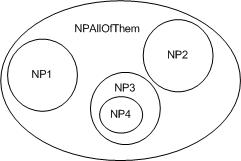
\includegraphics[bb=0 0 241 161, width=5.5in]{images/Nodepool1.jpg}
      \caption{Nodepool Example}
      \label{fig:Nodepools1}
    \end{figure}

    In the figure below the Nodepools are incorrectly defined for two reasons:
    \begin{enumerate}
       \item NP1 and NP2 overlap.
       \item NP4 overlaps both nodepool ``NpAllOfThem'' and NP3.
    \end{enumerate}
    
    \begin{figure}[H]
      \centering
      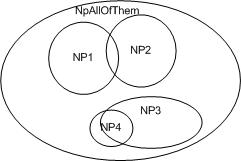
\includegraphics[bb=0 0 241 161, width=5.5in]{images/Nodepool2.jpg}
      \caption{Nodepools: Overlapping Pools are Incorrect}
      \label{fig:Nodepools2}
    \end{figure}

    Multiple ``top-level'' nodepools are allowed.  A ``top-level'' nodepool has no containing
    pool.  Multiple top-level pools logically divide a cluster of machines into {\em multiple
      independent clusters} from the standpoint of the scheduler.  Work scheduled over one
    pool in no way affects work scheduled over the other pool.  The figure below shows an
    abstract nodepool configuration with two top-level nodepools, ``Top-NP1'' and ``Top-NP2''.
    \begin{figure}[H]
      \centering
      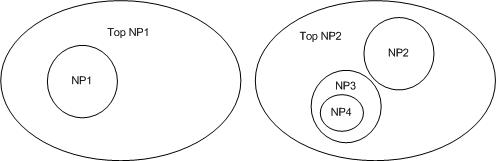
\includegraphics[bb=0 0 496 161, width=5.5in]{images/Nodepool3.jpg}
      \caption{Nodepools: Multiple top-level Nodepools}
      \label{fig:Nodepools3}
    \end{figure}

\subsubsection{Scheduling considerations}
    A primary goal of the scheduler is to insure that no resources are left idle if there
    is pending work that is able to use those resources.  Therefore, work scheduled to
    a class defined over a specific nodepool (say, NpAllOfThem), may be scheduled on nodes
    in any of the nodepools contained within NpAllOfThem.  If work defined over a
    subpool (such as NP1) arrives, processes on nodes in NP1 that were scheduled for
    NpAllOfThem are considered {\em squatters} and are the most likely candidates for
    eviction. (Processes assigned to their proper nodepools are considered {\em residents}
    and are evicted only after all {\em squatters} have been evicted.)  The scheduler strives
    to avoid creating {\em squatters}.

    Because non-preemptable allocations can't be preempeted, work submitted to a class
    implementing one of the non-preemptable policies (FIXED or RESERVE) are never allowed
    to ``squat'' in other nodepools and are only scheduled on nodes in their
    proper nodepool.

    In the case of multiple top-level nodepools: these nodepools and their subpools
    form independent scheduling groups.  Specifically,
    \begin{itemize}
        \item Fair-share allocations over any nodepool in one top-level pool do NOT affect the
          fair-share allocations for jobs in any other top-level nodepool. 

        \item Work submitted to classes under one top-level nodepool do NOT get expanded to
          nodes under another top-level nodepool, even is there is sufficient capacity.
    \end{itemize}

    Most installations will want to assign the majority of nodes to a single top-level
    nodepool (or its subpools), using other top-level pools for nodes that cannot be
    shared with other work.

\subsubsection{Configuration}
\label{subsubsec:nodepool.configuration}
    DUCC uses simple named stanzas containing key/value pairs to configure nodepools.

    At least one nodepool definition is required.  This nodepool need not have any subpools or node
    definitions.  The first top-level nodepool is considered the ``default'' nodepool.  Any node not
    named specifically in one of the node files which checks in with DUCC is assigned to this
    first, {\em default} nodepool. 

    Thus, if only one nodepool is defined with no other attributes, all nodes are
    assigned to that pool.

    A nodepool definition consists of the token ``Nodepool'' followed by the 
    name of the nodepool, followed by a block delimeted with ``curly'' braces \{ and \}.  This
    block contains the attributes of the nodepool as key/value pairs.
    Lineneds are ignored.  A semicolon ``$;$'' may optionally be used to
    delimit key/value pairs for readability, and an equals sign ``='' may optinally
    be used to delimit keys from values, also just for readability.  See the 
    \hyperref[fig:nodepool.configuration]{below}.

    The attributes of a Nodepool are:
    \begin{description}
      \item[domain] This is valid only in the ``default'' (first) nodepool.  Any node
        in any nodefile which does not have a domain, and any node which checks
        in to the Resource Manager without a domain name is assigned this domain name
        in order that the scheduler may deal entirely with full-qualified node names.

        If no {\em domain} is specified, DUCC will attempt to guess the domain based
        on the domain name returned on the node where the Resource Manager resides.

      \item[nodefile] This is the name of a file containing the names of the nodes
        which are members of this nodepool.

      \item[parent] This is used to indicate which nodepool is the logical parent.
        Any nodepool without a {\em parent} is considered a top-level nodepool.
    \end{description}
        
    The following example defines six nodepools, 
    \begin{enumerate}
      \item A top-level nodepool called ``--default--''.  All nodes not named
        in any nodefile are assigned to this nodepool.
      \item A top-level nodepool called ``jobdriver'', consisting of the nodes
        named in the file {\em jobdriver.nodes}.
      \item A subpool of ``--default--'' called ``intel'', consisting of the
        nodes named in {\em intel.nodes}.
      \item A subpool of ``--default--'' called ``power'', consisting of the
        nodes named in the file {\em power.nodes}.
      \item A subpool of ``intel'' called ``nightly-test'', consisting of the 
        nodes named in {\em nightly-test.nodes}.
      \item And a subpool of ``power'' called ``testing-p7'', consisting of the
        nodes named in {\em timing-ps.nodes}.
    \end{enumerate}

    \begin{figure}[H]
    
\begin{verbatim}
    Nodepool --default--  { domain bluej.net }
    Nodepool jobdriver    { nodefile jobdriver.nodes }
    
    Nodepool intel        { nodefile intel.nodes        ; parent --default-- }
    Nodepool power        { nodefile power.nodes        ; parent --default-- }

    Nodepool nightly-test { nodefile nightly-test.nodes ; parent intel }
    Nodepool timing-p7    { nodefile timing-p7.nodes    ; parent power }
\end{verbatim}
      \caption{Sample Nodepool Configuration}
      \label{fig:nodepool.configuration}

    \end{figure}    


    \subsection{Class Definitions}

    Scheduler classes are defined in the same simplified JSON-like language as
    nodepools.

    A simple inheritance (or ``template'') scheme is supported for classes.  Any
    class may be configured to ``derive'' from any other class.  In this case, the
    child class acquires all the attributes of the parent class, any of which may
    be selectively overridden.  Multiple inheritance is not supported but
    nested inheritance is; that is, class A may inherit from class B which inherits
    from class C and so on. In this way, generalized templates for the site's
    class structure may be defined.  

    The general form of a class definition consists of the keword Class, followed
    by the name of the class, and then optionally by the name of a ``parent'' class
    whose characteristics it inherits.   Following the name (and optionally parent class
    name) are the attributes of the class, also within a \{ blocak \} as for nodepools, and
    with lines and key/value pairs optionally delimeted by  ``$;$'' and ``$=$'', respectively.
    See the sample \hyperref[fig:class.configuration]{below}.

    The attributes defined for classes are:
    \begin{description}

      \item[abstract] If specified, this indicates this class is a template ONLY. It is used
        as a model for oher classes.  Values are ``true'' or ``false''.  The default is
        ``false''.  This class is never passed to the scheduler and may not be referenced
        by jobs.

      \item[cap] This specifies the largest number of shares that any job in this class
        may be assigned.  It may be an absolute number or a percentage.  If specified as
        a percentage (i.e. it contains a trailing \%), it specifies a percentage of the
        total nodes in the containing nodepool.

      \item[debug] FAIR\_SHARE only. This specifies the name of a class to substitute
        for jobs submitted for debug.  For example, if class {\em normal} specifies
\begin{verbatim}
     debug = fixed
\end{verbatim}
        then any job submitted to this class with debugging requested is actually scheduled
        in class {\em fixed}. (For example, one probably does not want a debugging job
        scheduled as FAIR\_SHARE and possibly preempted, preferring the non-preemptable
        class {\em fixed}.

      \item[default] This specifies the class to be used as the default class for work submission
        if no class is explicitly given.  Only one class of type FAIR\_SHARE may contain this
        designation, in which case it names the default FAIR\_SHARE class.  Only one class of type
        FIXED\_SHARE or RESERVE may contain this designation, in which case it names the default
        class to use for reservations (Note that either FIXED\_SHARE or RESERVE scheduling policies
        are valid for reservations.)

      \item[enforce] RESERVE only.  If specified, then reservations for this class must specify a
        memory size that exactly matches an eligible machine, modulo the share quanta.  For example,
        if the share quanta is 15G, a 15G reservation will never be honored on a 256G machine; in this
        case a 240G (or more) reservations must be specified.  The DUCC Web Server's {\em Machines} page
        displays the reccomended request size for every machine.  

        If {\em enforce} is not specified, the default is ``true''.

        If {\em enforce} is set to false, the scheduler will attempt to match the reservation as 
        closely as possible to an existing machine, and if it cannot it will use the next largest
        machine available.  Thus, a 15G reservation {\em might} be satisfied with a 240G machine if
        that is all that is available at the time.

      \item[expand-by-doubling] FAIR\_SHARE only.  If ``true'', and the {\em initialization-cap} is
        set, then after any process has initialized, the job will expand to its maximum allowable
        shares by doubling in size each scheduling cycle.  

        If not specified, the global value set in \hyperref[sec:ducc.properties]{ducc.properties} is used.

      \item[initialization-cap] FAIR\_SHARE only. If specified, this is the largest number of processes this job
        may be assigned until at least one process has successfully completed initialization.

        If not specified, the global value set in \hyperref[sec:ducc.properties]{ducc.properties} is used.

      \item[max-processes] FAIR\_SHARE and FIXED\_SHARE only.  This is the largest number of FIXED-SHARE,
        non-preemptable shares any single job may be assigned.

        Omit this property, or set it to 0 to disable the cap.

      \item[max-machines] RESERVE only.  This specifies the maximum number of full machines that
        may be reserved by any single job.

        Omit this property, or set it to 0 to disable the cap.

      \item[prediction-fudge] FAIR\_SHARE only. When the scheduler is considering expanding the
        number of processes for a job it tries to determine if the job may complete before those
        processes are allocated and initialized.  The {\em prediction-fudge} adds some amount of 
        time (in milliseconds) to the projected completion time.  This allows installations to
        prevent jobs from expanding when they were otherwise going to end in a few minutes
        anyway.

        If not specified, the global value set in \hyperref[sec:ducc.properties]{ducc.properties} is used.

      \item[nodepool] If specified, jobs for this class are assigned to nodes in this nodepool. The
        value must be the name of one of the configured nodepools.

      \item[policy] This is the scheduling policy, one of FAIR\_SHARE, FIXED\_SHARE, or RESERVE. This
        attribute is required (there is no default).

      \item[priority] This is the scheduling priority for jobs in this class.

      \item[weight] FAIR\_SHARE only. This is the fair-share weight for jobs in this class.
      
    \end{description}

    The following figure illustrates a representative class configuration for a large cluster,
    consisting of mixed Intel and Power nodes.  This class definition assumes the
    \hyperref[fig:nodepool.configuration]{nodepool configuration} shown above.  FAIR\_SHARE,
    FIXED\_SHARE, and RESERVE classes are defined over each machine architecture, Intel and Power,
    and over the combined pool. 

    \begin{figure}[H]    
\begin{verbatim}
# --------------------- Fair share definitions ---------------
Class fair-base {
      policy = FAIR_SHARE
      nodepool = intel
      priority = 10
      weight = 100
      abstract = true
      debug = fixed
}

Class nightly-test   fair-base  { weight = 100; nodepool nightly-test; priority = 7}

Class background     fair-base  { weight = 20 }
Class low            fair-base  { weight = 50 }
Class normal         fair-base  { weight = 100; default = true }
Class high           fair-base  { weight = 200 }
Class weekly         fair-base  { weight = 400 }

Class background-p7  background { nodepool = power }
Class low-p7         low        { nodepool = power }
Class normal-p7      normal     { nodepool = power }
Class high-p7        high       { nodepool = power }
Class weekly-p7      weekly     { nodepool = power }

Class background-all background { nodepool = --default-- }
Class low-all        low        { nodepool = --default-- }
Class normal-all     normal     { nodepool = --default-- }
Class high-all       high       { nodepool = --default-- }
Class weekly-all     weekly     { nodepool = --default-- }

# --------------------- Fixed share definitions ---------------
Class fixed-base {
      policy = FIXED_SHARE
      nodepool = intel
      priority = 5
      abstract = true
      max-processes = 10
}

Class fixed     fixed-base { }
Class fixed-p7  fixed-base { nodepool = power;    default = true; }
Class JobDriver fixed-base { nodepool = jobdriver; priority = 0 }      

# --------------------- Reserve definitions ---------------
Class reserve-base {
      policy = RESERVE
      nodepool = intel
      priority = 1
      enforce = true
      abstract = true
      max-machines = 10
}
 
Class reserve     reserve-base { }
Class reserve-p7  reserve-base { nodepool = power }
Class timing-p7   reserve-base { nodepool = timing-p7 }
\end{verbatim}
          \caption{Sample Class Configuration}
      \label{fig:class.configuration}
    \end{figure}
    
\subsection{Validation}

The administrative command, \hyperref[subsec:admin.check-ducc]{\em check\_ducc} may be used to
validate a configuration, with the {\em -c} option.  This reads the entire configuration and
nodefiles, validates consistency of the definitions and insures the nodepools do not overlap.

During startup, the \hyperref[subsec:admin.check-ducc]{\em start\_ducc} command always runs full validation, and if the
configuration is found to be incorrect, the cluster is not started.

Configuration checking is done internally by the DUCC java utility {\em
  org.apache.uima.ducc.commonNodeConfiguration}.  This utility contains a public
API as described in the Javadoc.  It may be invoked from the command line as follows:

    \paragraph{Usage:}
\begin{verbatim}
     java org.apache.uima.ducc.commonNodeConfiguration [-p] [-v nodefile] configfile
\end{verbatim}

    \paragraph{Options:}
    \begin{description}

      \item[$-p$] Pretty-print the compiled configuration to stdout. This illustrates
        nodepool nesting, and shows the fully-completed scheduling classes after inheritance.

      \item[$-v$ nodefile] This should be the master nodelist used to start DUCC.  This
        is assumed to be constructed to reflect the nodepool organization as 
        \hyperref[sec:admin-ducc.nodes]{described here}.  If provided,
        the nodepools are validated and checked for overlaps.

      \item[configfile] This is the name of the file containing the configuration.
    \end{description}
    

\section{Ducc Node Definitions}
\label{sec:admin-ducc.nodes}
    The DUCC node definitions are specified by default in the file {\em ducc.nodes}.

    The DUCC node list is used to configure the nodes used to run jobs and assign reservations. 
    When DUCC is started, the nodelist is read an a DUCC Agent is started on every node in the list.

    The node list can be composed of multiple node lists to assist organization of the DUCC cluster. 
    All the administrative commands operate upon node lists. By carefully organized these lists it is 
    possible to administer portions of a cluster independently. 

    In particular, it is highly recommended that the nodelists reflect the nodepool structure.  In
    this way, the configuration used to start DUCC is guaranteed to match the nodeppool definitions.

    Several types of records are permitted in nodelists:
    \begin{description}

      \item[Comments] A comment is delimited with the symbol ``$\#$''.  All text on the line
        following this symbol is ignored.

      \item[import] If a line starts with the symbol {\em import}, the next symbol on that line
        is expected to be the name of another node list.  This permits the DUCC cluster's
        nodes to be configured in a structured manner.

        For instance, the file {\em ducc.nodes} might consist entirely of {\em import} statements
        naming all of the nodepool files.
      \item[domain] This must be the first line of the file.  If specified, it should name
        the default domain to be used for all the nodes in this file, and the nodes named
        in imported files.  If not specified, then during start-up, nodes without domain names are assigned
        domain names according to the global domain name specified in the \hyperref[subsubsec:nodepool.configuration]{Resource Manager configuration}
        file, and if none is specified there, the domain name on the host starting DUCC is used.

      \item[nodename] This is a single token consisting of the name of a node on which an
        agent it to be started.

    \end{description}

    The example below shows a partial, hypothetical node configuration corresponding to the
    \hyperref[fig:nodepool.configuration]{nodepool configuration} above.

    \begin{figure}[H]

\begin{verbatim}
> cat ducc.nodes
# import all the nodes corresponding to my nodepools 
domain my.domain
import intel.nodes
import power.nodes
import jobdriver.nodes
import nightly-test.nodes
import timing-p7.nodes

> cat intel.nodes
# import the intel nodes, by frame
import intel-frame1.nodes
import intel-frame2.nodes
import intel-frame3.nodes

>cat intel-frame1.nodes
#import the specific nodes from frame1
r1s1node1
r1s1node2
r1s1node3
r1s1node4
\end{verbatim}
      \caption{Sample Node Configuration}
      \label{fig:node.configuration}

    \end{figure}    
    

% 
% Licensed to the Apache Software Foundation (ASF) under one
% or more contributor license agreements.  See the NOTICE file
% distributed with this work for additional information
% regarding copyright ownership.  The ASF licenses this file
% to you under the Apache License, Version 2.0 (the
% "License"); you may not use this file except in compliance
% with the License.  You may obtain a copy of the License at
% 
%   http://www.apache.org/licenses/LICENSE-2.0
% 
% Unless required by applicable law or agreed to in writing,
% software distributed under the License is distributed on an
% "AS IS" BASIS, WITHOUT WARRANTIES OR CONDITIONS OF ANY
% KIND, either express or implied.  See the License for the
% specific language governing permissions and limitations
% under the License.
% 
\section{DUCC Nodepool Definitions}

    REWRITE


%% This is a section
% 
% Licensed to the Apache Software Foundation (ASF) under one
% or more contributor license agreements.  See the NOTICE file
% distributed with this work for additional information
% regarding copyright ownership.  The ASF licenses this file
% to you under the Apache License, Version 2.0 (the
% "License"); you may not use this file except in compliance
% with the License.  You may obtain a copy of the License at
% 
%   http://www.apache.org/licenses/LICENSE-2.0
% 
% Unless required by applicable law or agreed to in writing,
% software distributed under the License is distributed on an
% "AS IS" BASIS, WITHOUT WARRANTIES OR CONDITIONS OF ANY
% KIND, either express or implied.  See the License for the
% specific language governing permissions and limitations
% under the License.
% 

\section{Administrative Commands}

   The administrative commands include a command to start DUCC, one to stop it, and one to 
   verify the configuration and query the state of the cluster.

   Note: The scripting that supports some of these functions runs (by default) in multi-threaded mode so
   large clusters can be started, stopped, and queried quickly.  If DUCC is running on an older
   system, the threading may not work right, in which case the scripts detect this and run
   single-threaded.  As well, all these commands support a ``--nothreading'' option to manually
   disable the threading.

\subsection{start\_ducc}
\label{subsec:admin.start-ducc}

    \subsubsection{{\em Description}}
    The command \ducchome/admin/start\_ducc is used to start DUCC processes. 
    It must be run from the head node.
    If run with no parameters it takes the following actions:
    \begin{itemize}
      \item Starts the ActiveMQ server.
      \item Starts the database.
      \item Starts the management processes Resource Manager, Orchestrator, Process Manager,      
      Services Manager, and Web Server on the local node.
      \item Starts an agent process on every node named in the default node list. 
    \end{itemize}

    \subsubsection{{\em Usage}}

    \begin{description}
      \item[start\_ducc {[options]}] \hfill \\ 
        If no options are given, all DUCC processes are started, using the default node list, 
        {\em ducc.nodes}. 
      
      \end{description}
      
      \subsubsection{{\em Options: }}
      \begin{description}

        \item[-n, --nodelist {[nodefile] }] \hfill \\
          Start agents on the nodes in the nodefile. Multiple nodefiles may be specified: 
\begin{verbatim}
start\_ducc -n foo.nodes -n bar.nodes -n baz.nodes 
\end{verbatim}
          

        \item[-c, --component {[component] }] \hfill \\
          Start a specific DUCC component, optionally on a specific node. If the component 
          name is qualified with a nodename, the component is started on that node. To qualify 
          a component name with a destination node, use the notation component@nodename. 
          Multiple components may be specified: 
\begin{verbatim}
start\_ducc -c sm -c pm -c rm -c or@bj22 -c agent@n1 -c agent@n2 
\end{verbatim}
          
          Components include: 
          \begin{description}
            \item[rm] The Resource Manager
            \item[or]The Orchestrator
            \item[pm]The Process Manager
            \item[sm]The Service Manager
            \item[ws]The Web Server
            \item[agent@node]Node Agents
            \item[broker] ActiveMQ broker
            \item[db] Database
          \end{description}

          \item[--nothreading] If specified, the command does not run in multi-threaded mode
            even if it is supported on the local platform.

      \end{description}

      \subsubsection{{\em Notes: }}
      A different nodelist may be used to specify where Agents are started. As well multiple node 
      lists may be specified, in which case Agents are started on all the nodes in the multiple node 
      lists. 
      
      To start only agents, run start\_ducc specifying a nodelist explicitly. Note that the broker
      must have already been started.
      
      To start a specific management process, run start\_ducc with the -c component parameter, 
      specify the component that should be started. 
      
      \subsubsection{{\em Examples: }}

      Start some nodes from two different nodelist and start the broker.  
\begin{verbatim}
        start\_ducc -n foo.nodes -n bar.nodes -c broker
\end{verbatim}
                  
      Start an agent on a specific node: 
\begin{verbatim}
        start\_ducc -c agent@a.specific.node 
\end{verbatim}
      
      Start the webserver on node 'bingle': 
\begin{verbatim}
        start\_ducc -c ws@bingle 
\end{verbatim}

      \subsubsection{{\em Debugging:}}

      Sometimes something will not start and it can be difficult to understand why.  To diagnose, it is
      helpful to know that {\em start\_ducc} is simply a wrapper around a lower-level bit of scripting
      that does the actual work.  That lower-level code can be invoked stand-alone, in which case
      console messages that {\em start\_ducc} will have suppressed are presented to the console.

      The lower-level script is called {\em ducc.py} and accepts the same {\em -c component} flag as
      start\_ducc.  If some component will not start, try running {\em ducc.py -c component} directly.
      It will start in the foreground and usually the cause of the problem becomes evident from
      the console.

      For example, suppose the Resource Manager will not start.  Run the following:
\begin{verbatim}
      ./ducc.py -c rm
\end{verbatim}
      and examine the output.  Use {\em CTL-C} to stop the component when done.
      

\subsection{stop\_ducc}
\label{subsec:admin.stop-ducc}

    \subsubsection{{\em Description:}}
    Stop\_ducc is used to stop DUCC processes. At least one parameter is required.
    When {\em -a} is specified, the following actions are taken:
    \begin{itemize}
       \item Uses the ActiveMQ broker to broadcast a shutdown request to all
        DUCC compoments, other than the ActiveMQ broker itself, and the database.
      \item Waits a bit, for all daemons to stop.
      \item Stops the database.
      \item Stops the ActiveMQ broker.
    \end{itemize}


    \subsubsection{\em Usage:}

    \begin{description}
      \item[stop\_ducc {[options]}] \hfill \\ 
        If no options are given, help text is presented. At least one option is required, to avoid 
        accidental cluster shutdown. 
      \end{description}
    

      \subsubsection{Options:}
        \begin{description}

          \item[-a --all] \hfill \\
            Stop all the DUCC processes, including agents and management processes. This 
            broadcasts a "shutdown" command to all DUCC processes. Shutdown is normally 
            performed gracefully with all processes given time to save state. 
            All user processes, both jobs and services, are sent shutdown signals. Job and service 
            processes which do not shutdown within a designated grace period are then forcibly 
            terminated with kill -9. 
            
          \item[-n, --nodelist {[nodefile]}] \hfill \\
            Only the DUCC agents in the designated nodelists are shutdown. The processes are sent 
            kill -INT signals which triggers the Java shutdown hooks and enables graceful shutdown. 
            All user processes on the indicated nodes, both jobs and services, are sent "shutdown" 
            signals and are given a minute to shutdown gracefully. Job and service processes which do 
            not shutdown within a designated grace period are then forcibly terminated with kill -9. 
            
\begin{verbatim}
stop\_ducc -n foo.nodes -n bar.nodes -n baz.nodes 
\end{verbatim}

          \item[-c, --component {[component]}] \hfill \\
            Stop a specific DUCC component. 

            This may be used to stop an errant management component and subsequently restart it 
            (with start\_ducc). 
            
            This may also be used to stop a specific agent and the job and services processes it is
            managing, without the need to specify a nodelist.  
            
            Examples: 

            Stop agents on nodes n1 and n2:
\begin{verbatim}
stop_ducc -c agent@n1 -c agent@n2 
\end{verbatim}
            
            Stop and restart the rm: 
\begin{verbatim}
stop_ducc -c rm 
start_ducc -c rm
\end{verbatim}
            
            Components include: 
            \begin{description}
              \item[rm] The Resource Manager.                 
              \item[or] The Orchestrator.                 
              \item[pm] The Process Manager.                 
              \item[sm] The Service Manager.                 
              \item[ws] The Web Server.                 
              \item[db] The database.
              \item[broker] The ActiveMQ broker (only if the broker is auto-managed).
              \item[agent@node] Node Agent on the specified node.
              \end{description}

          \item[-w, --wait {[time in seconds]}] If given, this signals the time to wait
            after broadcasting the shutdown signal, and before stopping the ActiveMQ broker itself.
            If not specified, the default is 60 seconds.  

            NOTE: In production systems, it is generally wise to use the default of 60 seconds.  For
            test systems a shorter wait speeds cycle time.  Be sure to use {\em check\_ducc -k} after
            {\em stop\_ducc} if you change the wait time to insure all processes are actually stopped.

          \item[--nothreading] If specified, the command does not run in multi-threaded mode
            even if it is supported on the local platform.
              
       \end{description}
            
   \subsubsection{{\em Notes:}}
   Sometimes problems in the network or elsewhere prevent the DUCC components from stopping properly.  The
   {\em check\_ducc} command, described in the following section, contains options to query the
   existance of DUCC processes in the cluster, to forcibly ({\em kill -9}) terminate them, and to
   more gracefully terminate them ({\em kill -INT}).
          


\subsection{check\_ducc}
\label{subsec:admin.check-ducc}
    \subsubsection{{\em Description:}}

    Check\_ducc is used to verify the integrity of the DUCC installation and to find and report on
    DUCC processes. It identifies processes owned by ducc (management processes, agents,
    and job processes), and processes started by DUCC on behalf of users.
    
    Check\_ducc can also be used to clean up errant DUCC processes when stop\_ducc is unable 
    to do so. The difference is that stop\_ducc generally tries more gracefully stop processes. 
    check\_ducc is used as a last resort, or if a fast but graceless shutdown is desired. 
    
    \subsubsection{\em{Usage: }}

        \begin{description} 
          \item[check\_ducc {[options]}]
              If no options are given this is the equivalent of: 
\begin{verbatim}
check_ducc -c -n ../resources/ducc.nodes 
\end{verbatim}
              
              This verifies the integrity of the DUCC installation and searches for all the
              processes owned by user {\em ducc} and started by DUCC on all the nodes in ducc.nodes.
        \end{description}
            
     \subsubsection{\em{Options:}}
         \begin{description}
           \item[-n --nodelist {[nodefile]}]
             Only the nodes specified in the nodefile are searched. The option may be specified 
             multiple times for multiple nodefiles. Note that the "local" node is always checked as well. 
\begin{verbatim}
check_ducc -n nlist1 -n nlist2 
\end{verbatim}
                       
           \item[-c --configuration]
             Verify the \hyperref[sec:ducc.classes]{Resource Manager configuration}.

           \item[-p --pids]               
               Rewrite the PID file. The PID file contains the process ids of all known DUCC 
               management and agent processes. The PID file is normally managed by start\_ducc and 
               stop\_ducc and is stored in the file {\em ducc.pids} in directory {\em ducc\_runtime/state}.
               
               Occasionally the PID file can become partially or fully corrupted; for example, if a DUCC 
               process dies spontaneously. Use check\_ducc -p to search the cluster for processes and 
               refresh the PID file. 
               
            \item[-i, --int] \hfill \\
              Use this to send a shutdown signal ({\em kill -INT}) to all the DUCC processes.  The DUCC processes
              catch this signal, close their resources and exit.  Some resources take some time to close, or in
              case of problems, are unable to close, in which case the DUCC processes will unconditionally exit.

              Sometimes problems in the network or elsewhere prevent {\em check\_ducc -i} from terminating
              the DUCC processes.  In this case, use {\em check\_ducc -k}, described below.

            \item[-k, --kill] \hfill \\
              Use this to forcibly kill a component using kill -9. This should only be used if {\em stop\_ducc}
              or {\em check\_ducc -i} does not work.  

            \item[--nothreading] If specified, the command does not run in multi-threaded mode
              even if it is supported on the local platform.

            \item[-v, --verbose] \hfill \\
              When specified with {\em -c} to check the configuration, this emits a formatted version
              of the node list showing the full structure of the scheduling classes.
              

           \end{description}               


            
\subsection{build\_duccling}
\label{subsec:admin.build-duccling}

    See ~\ref{sec:duccling.install} on Ducc\_ling Configuration.


\subsection{ducc\_disk\_info}
\label{subsec:admin.ducc-disk-info}
    \subsubsection{{\em Description:}}

    The disk info tool is used to obtain information about DUCC disk usage. 
    
    \paragraph{Usage:}
        This command nominally takes no parameters.
        
    \paragraph{Options:}
    \begin{description}
      	\item -h, --help      Prints the usage text to the console. 
      	\item -c, --code      Prints the exit code, which is the greater of disk usage percentage and quota usage percentage. 
      	\item -d, --debug     Prints internal debugging information, intended for DUCC developers or extended problem determination.
      	\item -n, --nomsg     Suppress display of filesystem and quota percentages used message. 
    \end{description}       


\subsection{ducc\_gather\_logs}
\label{subsec:admin.ducc-gather-logs}
    \subsubsection{{\em Description:}}

    Purpose: gather problem determination information comprising DUCC logs and configuration data into a gz file.
    
    \paragraph{Usage:}
        This command nominally takes no parameters.
        
    \paragraph{Options:}
    \begin{description}
      	\item -h, --help      Prints the usage text to the console. 
      	\item -d DIRECTORY, --directory DIRECTORY     Path to directory for gz file, default=/tmp.
    \end{description}       
    

\subsection{ducc\_post\_install}
\label{subsec:admin.ducc-post-install}

    \paragraph{Description:}
    The post-installation script must be run only after the first installation of DUCC. 
    When updating an existing installation use \hyperref[subsec:admin.ducc-update]{\em ducc\_update}.
    ducc\_post\_install performs these tasks:
    \begin{enumerate}
      \item Verifies that the correct level of Java and Python are installed and available.
      \item Creates a default nodelist, \duccruntime/resources/ducc.nodes, containing the name of the node you are installing on.
      \item Defines the ``ducc head'' node to be the node you are installing from.
      \item Initializes the database.
      \item Sets up the default https keystore for the webserver.
      \item Installs the DUCC documentation ``ducc book'' into the DUCC webserver root.
      \item Builds and installs the C program, ``ducc\_ling'', into the default location.
      \item Ensures that the (supplied) ActiveMQ broker is runnable.
    \end{enumerate}

    Once the script completes successfully \hyperref[subsec:admin.start-ducc]{\em start\_ducc} will run a single-user/unprivileged DUCC.

    \paragraph{Notes:}
    If the script is rerun it will rename the previously created files so any customizations applied
    can be recovered.

\subsection{ducc\_update}
\label{subsec:admin.ducc-update}

    \paragraph{Description:}
        This command is used to unpack a new release of DUCC and create a new installion or update
        an existing one.
        For a new installation it simply unpacks the tar file with the appropriate permissions.
        The setup must be completed by running \hyperref[subsec:admin.ducc-post-install]{\em ducc\_post\_install}.

        When updating an existing installation it performs the following actions:
        \begin{enumerate}
          \item Checks that DUCC is not running.
          \item Creates a site.ducc.properties file if updating from DUCC 1.1.0.
          \item Creates a time-stamped archive directory to hold the old runtime.
          \item Archives current files before updating them, except for the customizable ones.
          \item Leaves in place any files added to the directories that may hold csite-specific files.
          \item Reports which are replaced, added, or kept.
          \item Rebuilds the non-privileged ducc\_ling.
        \end{enumerate}

        The site-specific files, those holding customizations such as node and class definitions
        as well as logs and job history, are left in place, 
        while all replaced files are archived under a folder called {\em ducc\_archives} 
        so the previous installation can be restored if necessary.

        Note that the update does not create the database.  After updating to 2.1.0 from an earlier
        version with the file-based persistent scheme the database should be created with
        \hyperref[subsec:admin.db-create]{\em db\_create} 
        and the files holding state such as job history and service registrations loaded into the database with
        \hyperref[subsec:admin.db-loader]{\em db\_loader}.
        If this conversion is omitted DUCC will continue to use the file-based scheme but with some
        loss of functionality that the database design would provide.
        
    \paragraph{Usage:}
        This command takes two parameters, a pointer to the DUCC\_HOME to be updated or created,
        and the name of the tar file containg the new build.
    \begin{description}
      \item[ducc\_update {\em some-ducc-home} {\em binary-tar-file}]
        Update an existing DUCC installation or install a new one.
    \end{description}

    \paragraph{Arguments:}
    \begin{description}
        \item[{\em some-ducc-home}] 
          This specifies the DUCC\_HOME you wish to create or update.  If it doesn't exist a new
          installation is created, otherwise it is updated.
        \item[{\em binary-tar-file}]
          The name of the binary tar file containing the new build.
     \end{description}

    \paragraph{Example:}
\begin{verbatim}
ducc_update ducc_runtime /home/ducc/ducc_runtime Downloads/uima-ducc-2.1.0-bin.tar.gz 
\end{verbatim}


\subsection{move\_ducc}
\label{subsec:admin.move-ducc}

    \paragraph{Description:}
        This command is used to move the DUCC head node from one node to another.
        Run this command on the node which is to become the new DUCC head node.

        It performs the following actions:
        \begin{enumerate}
          \item Checks that DUCC is not running.
          \item Insures that the new DUCC head node is in the ducc.head.failover list.
          \item Creates a backup of the site.ducc.properties file.
          \item Updates the site.ducc.properties file with revised head and database entries.
          \item Indicates that move operation is completed.
        \end{enumerate}

        Nominally, the manual steps to move the DUCC head node are:
        \begin{enumerate}
          \item Issue stop\_ducc command on the current DUCC head node.
          \item Issue move\_ducc command on the new DUCC head node.
          \item Issue start\_ducc command on the new DUUCC head node.
        \end{enumerate}

        Note that the stop\_ducc command can be issued with either the 
        {\em --all}
        or the 
        {\em -c head}
        options.
        In the later case, existing work will continue to the extent possible.
               
        The move\_ducc command requires that:
        \begin{enumerate}
          \item The command itself must be issued on the new DUCC head node.
          \item The old DUCC head node is up.
          \item The old DUCC head node daemons are down.
          \item The old DUCC head node and new DUCC head node are not the same.
          \item The old DUCC head node and old DUCC database node matrch site.ducc.properties.
          \item The new DUCC head node is in the ducc.head.failover list in site.ducc.properties.
          \item If the old DUCC head node is down, then the --offline parameter must be specified.
        \end{enumerate}
       
    \paragraph{Usage:}
        This command nominally takes no parameters.
        
    \paragraph{Options:}
    \begin{description}
      	\item -h, --help     show this help message and exit
      	\item -d, --debug    display debugging messages
      	\item -o, --offline  indicate current DUCC head node is offline, Note: USE THIS OPTION WITH EXTREME CAUTION else risk corrupting database
      	\item -q, --quiet    do not display informational messages
    \end{description}

    \paragraph{Example:}
\begin{verbatim}
move\_ducc 
\end{verbatim}


\subsection{rm\_reconfigure}
\label{subsec:admin.rm-reconfigure}

    \subsubsection{{\em Description:}}
    Rm\_reconfigure is used to force the Resource Manager (RM) to reread all its configuration
    files and reconfigure itself accordingly, without the need to fully stop and restart RM.
    This is generally much faster than RM restart and avoids losing most state messages from
    the other DUCC processes.
    
    The {\em rm\_reconfigure} command first performs a 
    \hyperref[sec:admin.properties-merge]{properties merge.}

    RM then validates the new
    configuration, and if no errors are found, saves certain information such as current node
    online-offline status.  It then rereads the following configuration files and rebuilds its
    internal structures accordingly:
    \begin{itemize}
      \item ducc.properties (after merging default.ducc.properties and site.ducc.properties,
      \item ducc.classes,
      \item log4j.xml.
    \end{itemize}
    The saved configuration is then restored into the newly configured structures.
    On receipt of the next Orchestrator state, the RM fully rebuilds its state from the current
    DUCC load and scheduling restarts.

    Depending on the nature of the new configuration, the current load may be adjusted; for
    example, if the weight of a fair-share class is changed, preemptions or extra allocations
    may be performed.

    If the new configuration is not consistent with the current load, a number of more drastic
    adjustments will be performed:
    \begin{itemize}
      \item If a fair-share class is deleted, all existing jobs for that class are preempted
        and a {\em refusal} message is sent to the Orchestrator for each affected job.
      \item If a fair-share class is redefined over a different nodepool such that existing
        work are no longer legally scheduled, any shares allocated over inappropriate
        hosts are {\em preempted}.  As soon as the preemptions are acknowledged, the RM
        will reschedule the shares over the differently-configured resources.
      \item If a non-preemptable class is deleted or reconfigured so existing non-preempt able
        work is no longer allocated correctly, the following will occur:
        \begin{itemize}
            \item If the shares are for services, they are deallocated and a {\em refusal} is
              sent to the Orchestrator.  The Service Manager will observe this and restart the
              processes, causing them to be reallocated over the changed configuration.
            \item Otherwise, the RM leaves the allocation in place, but places the hosts on an
              internal {\em blacklist}, preventing subsequent scheduling to those hosts. Once
              the (now) incorrectly placed shares are freed (e.g. by canceling a reservation or
              exit of a managed reservation), the hosts are again white listed and made available
              for scheduling.
        \end{itemize}
     \end{itemize}
        
    In short, the RM makes every effort to avoid disturbing existing allocations, and blacklists
    hosts that are no longer consistently configured for the current load, until such time as
    the allocations on those hosts are released.

    \subsubsection{\em Usage:}

    \begin{description}
      \item[rm\_reconfigure] \hfill \\ 
        This command has no options.
      \end{description}
             
       
\iffalse  % Dropped this script for 2.1 .... needs work

\subsection{rm\_qload}
\label{subsec:admin.rm-qload}

    \subsubsection{{\em Description:}}
    Rm\_qload is used to query the Resource Manager's scheduling tables to determine the
    current demand and capacity of the system, as the RM sees it.  The primary purpose
    is to provide information to adjunct resource managers (such as a ``cloud'') to
    determine the current needs, or lack thereof, of the system.  The administrative
    command is implemented as a Python script that interacts with the underlying
    Java ``RmQueryLoadReply'' API and is provided mostly as an example of how
    scripting can be used to interact with the RM.

    After displaying the current scheduling quantum, the response is provided in two sections:
    \begin{enumerate}
      \item Information showing the current demand and usage of resource classes, and
      \item Information showing the current nodepool usage.
    \end{enumerate}

    \subsubsection{\em Class section}
    Three lines are emitted per class:
    \begin{enumerate}
      \item The name of the class and its scheduling policy,
      \item A line showing the {\em demand}, or {\em request} by quantum, on the class, and
      \item A line showing the {\em usage}, or {\em award}, by quantum on the class.
    \end{enumerate}
    
    The numbers shown for {\em request} and {\em award} show the number of processes, by
    memory, in terms of scheduling quantum, for each class.  For example, assuming the
    scheduling quantum is 15GB, the following shows:
    \begin{itemize}
      \item Five processes of quantum 2 (15-30GB) are requested, but only two have been awarded,
      \item Three processes of quantum 3 (31-45GB) are requested and all have been awarded,
      \item Four processes of quantum 4 (46-60GB) are requested, and two have been awarded.
    \end{itemize}
\begin{verbatim}
Class normal policy FAIR_SHARE
   requested    0    0    5    3    4    0    0    0    0 
   awarded      0    0    2    3    2    0    0    0    0 
\end{verbatim}

    \subsubsection{\em Nodepool section}
    Six lines are displayed for each nodepool:
    \begin{enumerate}
      \item The name of the nodepool,
      \item A summary showing the number hosts in the pool which are online, dead (unresponsive), and
          varied-off, the total quantum shares available to the nodepool, and the total unscheduled or 
          {\em free} shares.
      \item The number of hosts known to the nodepool, by quantum, similar to the class listings above,
      \item The nubmer of online hosts, by quantum,
      \item The number of completely free hosts by quantum (no work currently scheduled), and
      \item The number of {\em virtual} hosts, by quantum.  A {\em virtual host} is created when a
          host is partially scheduled.  For example, if a 32G processes is scheduled on a 64G host, this
          creates one free 32G {\em virtual host}.
    \end{enumerate}
    To determine the number of processes, by quantum, that can be scheduled, one must {\em sum} the
    ``free'' and ``virtual'' columns.
    
    For example, (assuming a 15GB quantum), the following listing shows
    that nodepool ``power'' contains fourteen hosts with at least 45GB each (3 quanta).  Two
    of these hosts have something scheduled on them (the ``free
    machines'' line), leaving unused space of one 15G quantum on one
    host, and one 30GB quantum on another host.

\begin{verbatim}
Nodepool power
   online 14 dead 0 offline 0 total-shares 42 free-shares 42
   all     machines:    0    0    0   14    0    0    0    0    0 
   online  machines:    0    0    0    0    0    0    0    0    0 
   free    machines:    0    0    0   12    0    0    0    0    0 
   virtual machines:    0    1    1    0    0    0    0    0    0 
\end{verbatim}

    \subsubsection{\em Usage:}
    \begin{description}
      \item[rm\_qload] \hfill \\ 
        This command has no options.
      \end{description}

\fi     % End of dropped rm_qload         
       
\subsection{rm\_qoccupancy}
\label{subsec:admin.rm-qoccupancy}

    \subsubsection{{\em Description:}}
    Rm\_qoccupancy provides a list of all known hosts to the RM, and for each host, the following information:
    \begin{itemize}
      \item The name of the host,
      \item Whether the host has any blacklists processes on it,
      \item Whether the host is currently onlline (responsive),
      \item The status of the host; whether the host is schedulable ({\em up} or {\em down}.  A responsive host becomes
        unschedulable ({\em down}) if it is varied-off,
      \item The nodepool the host is a member of,
      \item The reported memory size of the host, 
      \item The {\em order} of the host.  The {\em order} is defined to be the maximum number of quantum shares
        supported by the host,
      \item The number of unscheduled quantum shares on the host, and
      \item If work is scheduled on the host, information relevent to that scheduled processes (or reservation).
    \end{itemize}

    If work is scheduled on a host, the work summary is keyed thus:
    \begin{description}
      \item[J] The Orchestrator-assigned job id of the work,
      \item[S] The RM-assigned share id of the work,
      \item[O] The {\em order} of the allocation; that is, the number of quantum shares the allocation occupies,
      \item[II] The {\em initialization investment}; the number of milliseconds the allocated work spent in its
        initialization phase, if any (usually only UIMA-AS processes display this),
      \item[IR] The {\em runtime investment}; the number of milliseconds spent processing the current CASs, if this
        is a UIMA-AS processes.  Note that this number can change dramatically, as it is the sum of time spent only
        by the current CASs.  When a CAS completes, it no longer contributes to the investment of the process.  The RM
        uses this information to determine the best candidate for eviction, if needed ot maintain fair-share.
      \item[E] Whether the RM has preempted (evicted) the process but it has not yet exited,
      \item[P] Whether the RM has purged the process (evicted, because the host is non-responsive), but it has not
        been confirmed evicted,
      \item[F] Whether the process is {\em fixed}; that is, non-preemptbable,
      \item[I] Whether the initialization phase is completed (usually only UIMA-AS processes).
    \end{description}

    The following example shows seven hosts, one with a preemptable share in the {\em --default--}
    nodepool (on bluej290-5), and one with a non-preemptable share in the {\em jobdriver} nodepool.
\begin{verbatim}
        Node Blacklisted Online Status        Nodepool     Memory Order   Free
  bluej290-5       False   True     up     --default--   32505856     2      0
            J[    6006] S[     189] O[2] II[       0] IR[       0] E[False] P[False] F[False] I[False]

  bluej290-6       False   True     up     --default--   32505856     2      2
  bluej290-7       False   True     up     --default--   32505856     2      2
 bluej291-26       False   True     up    nightly-test   32505856     2      2
 bluej291-27       False   True     up    nightly-test   32505856     2      2
 bluej293-60       False   True     up           intel   32505856     2      2
 bluej537-73       False   True     up       jobdriver   32505856     2      1
            J[    5973] S[       1] O[1] II[       0] IR[       0] E[False] P[False] F[ True] I[False]


\end{verbatim}


    \subsubsection{\em Usage:}

    \begin{description}
      \item[rm\_qoccupancy] \hfill \\ 
        This command has no options.
      \end{description}
             
       

\subsection{vary\_off}
\label{subsec:admin.vary-off}
    \subsubsection{{\em Description:}}

    Vary\_off is used to remove a host from scheduling and to evict the preemptable work that is running on it.
    This allows for graceful clearance of a host so the host can be take offline for maintenance,
    or any other purpose (such as sharing the host with other applications.)  
    The DUCC agent is NOT stoppped; use \hyperref[subsec:admin.stop-ducc]{stop\_ducc} to stop the
    agent.  
    Managed and unmanaged reservations are not canceled by {\em vary\_off}.
    
    Only the userid that started DUCC may issue {\em vary\_off}; attempts from other userids
    are rejected.

    \subsubsection{\em{Usage: }}

        \begin{description} 
          \item[vary\_off list-of-hosts]
            The {\em list-of-nodes} is a space delimited list of hosts to be removed from
              scheduling in the DUCC cluster.
        \end{description}
            
\subsection{vary\_on}
\label{subsec:admin.vary-on}
    \subsubsection{{\em Description:}}

    Vary\_on is used to restore a host to scheduling by DUCC.  If the agent is still
    alive the host becomes immediately available.  The agent is not started by
    {\em vary\_on}; use use 
    \hyperref[subsec:admin.start-ducc]{start\_ducc} to start the agent if needed.

    Only the userid that started DUCC may issue {\em vary\_on}; attempts from other userids
    are rejected.
    
    \subsubsection{\em{Usage: }}

        \begin{description} 
          \item[vary\_on list-of-hosts]
            The {\em list-of-nodes} is a space delimited list of hosts to be restored for
              scheduling in the DUCC cluster.
        \end{description}
            
       
\subsection{ducc\_properties\_manager}
\label{sec:cli.ducc-properties-manager}

    \paragraph{Description:}
    This CLI is used to manually merge or difference two properties files. 

    Normally, the DUCC scripts {\em start\_ducc, check\_ducc,}, and {\em rm\_configure} automatically
    merge the file {\em default.ducc.properties} and {\em site.ducc.properties} when invoked.  

    \paragraph{Usage:}
    \begin{description}
    \item[ducc\_props\_manager --merge file1 --with file2 --to file3]
      Merge two properties files into one.  Properties added to, or changed in, the second file
      are used to override those in the first file, with the result written to the third file.
    \item[ducc\_props\_manager --delta file1 --with file2 --to file3]
      Compare two properties files and write the differences into a third file.  The first file is
      considered a ``master'' file.  Properties with different values in the second file, or which
      do not occur in the first file, are written into the third file.
    \end{description}

    \paragraph{Options:}
    \begin{description}
        \item[$--$merge file1]          
          In this form, the two files specified in the {\em $--$with} and {\em$--$to} fields are merged, with the
          results placed in $--$file3.  Overrides are flagged with a change tag and the date of the merge.

          {\em file1} is considered the ``master'' properties file and is usually the unmodified file provided
          with the DUCC distribution, {\em default.ducc.properties}.

          {\em file2} is considered a set of override or additional properties and is usually the site local
          properties file, {\em site.ducc.properties.}

        \item[$--$delta file1]
          In this form, the two files specified in the {\em $--$with} and {\em$--$to} fields are compared, with
          differences placed in $--$file3.

          {\em file1} is considered the ``master'' properties file and is usually the unmodified file provided
          with the DUCC distribution, {\em default.ducc.properties}.
          
          {\em file2} is considered the ``external'' properties file and is usually the properties file from
          an older version of DUCC.  

          Differences are placed in {\em $--$file3} which may be a viable first cut at a new {\em site.ducc.properties.}

          \item[$--$with file2] This specifies the properties file to merge with the master, or to difference
            with the master properties file.

          \item[$--$to file3] This specifies the file to which the results of the merge or delta are written.
     \end{description}
        
    \paragraph{Notes:}
    None.

\subsection{db\_create}
\label{subsec:admin.db-create}

    \paragraph{Description:}
        This command is used to initialize the database.  Normally the database is initialized
        during {\em ducc\_post\_install} but if this is an existing DUCC installation that is 
        being migrated from a version that does not use the database, it will be necessary to
        initialize the database with this command.

        This command performs the following actions:
        \begin{enumerate}
          \item Starts the database.
          \item Disables the default database superuser.
          \item Installs a database superuser as ``ducc'' and sets the password
            to a random string.  The password is saved
            in DUCC\_HOME/resources.private/ducc.private.properties.
          \item Installs the DUCC database schema.
          \item Stops the database.
        \end{enumerate}
        

         This command takes no parameters.

         NOTE: The database user and password are NOT RELATED to any login ID on the system,
         they are used and maintained by the database only.

\subsection{db\_loader}
\label{subsec:admin.db-loader}

    \paragraph{Description:}
        This command is used to copy the data from DUCC's older (pre 2.1.0) file-based persistence
        into the database.  The database schema must already exist, created either
        with {\em ducc\_post\_install} or with {\em db\_create}.

        This command performs the following actions:
        \begin{enumerate}
          \item Starts the database.
          \item Drops some of the indexes in the database.
          \item Loads the Orchestrator checkpoint file from {\em DUCC\_HOME/state/orchestrator.chkpt}.
          \item Loads all job history from {\em DUCC\_HOME/history/jobs}.
          \item Loads all reservation history from {\em DUCC\_HOME/history/reservations}.
          \item Loads all service instance and AP history from {\em DUCC\_HOME/history/services}.
          \item Loads the service registry from {\em DUCC\_HOME/state/services}.
          \item Loads the service registry histroy from {\em DUCC\_HOME/history/service-registry}.  
          \item Reloads the Orchestratory checkpoint, as a spot-check of the loader's instrumentation (to insure
            load times stay reasonable.)
          \item Re-installs the DUCC database schema.
          \item Stops the database.
          \item Optionally renames the file-based state so if you rerun the command, the data does not get reloaded.
        \end{enumerate}
        
        When the command exits, DUCC should be ready to run with all its state in the database.

        This command takes two parameters, a pointer to the DUCC\_HOME you want to load from, and
        a flag to disable the rename of the file-based state.

    \paragraph{Usage:}
    \begin{description}
    \item[db\_loader -i {\em some-ducc-home} {[--no-archive]}]
      Load the database from the specified DUCC\_HOME, and optionally do not archive the original files
      by renaming them.  
    \end{description}

    \paragraph{Options:}
    \begin{description}
        \item[$-i$ {\em some-ducc-home}] 
          This specifies the DUCC\_HOME you wish to load.  Most of the time it is the DUCC\_HOME you
          are running within, but it can be some other DUCC\_HOME if you have multiple installations and
          want other history and state loaded.
        \item[$--no-archive$] 
          If specified, the original files are not renamed.  Note that only the directories in {\em history}
          and {\em state} are renamed.  To restore these, simply rename them back without the {\em archive}
          suffix.
     \end{description}
        
    \paragraph{Example:}
\begin{verbatim}
db_loader -i /home/ducc/ducc_runtime
db_loader -i /home/ducc.old/ducc_runtime --no-archive
\end{verbatim}

    \paragraph{Notes:}
    The console shows progress of the loader.  Full details of the load are written to a log {\em db-loader-log}
    in the usual DUCC log directory, for reference and potential problem determination if something goes wrong.
    
    
\subsection{db\_tool}
\label{subsec:admin.db-tool}

    \paragraph{Description:}
        This command is used to backup and restore DUCC's database.
        
    \paragraph{Options:}
    Exactly one of the following options is required.
    \begin{description}
	        \item[$--save$ {\em PATH.tar.gz}] 
	          The file to save the DUCC database contents.  The database must be up.  The file cannot already exist.
       		\item[$--save-overwrite$ {\em PATH.tar.gz}] 
	          The file to save the DUCC database contents.  The database must be up.
	        \item[$--restore$ {\em PATH.tar.gz}] 
	          The file to restore the DUCC database contents.  The database must be down.  The database directory cannot exist.
	        \item[$--restore-overwrite$ {\em PATH.tar.gz}] 
	          The file to restore the DUCC database contents.  The database must be down.
     \end{description}
	 The following options are optional and are mutually exclusive wtih each other.
	 \begin{description}
	        \item[$--verbose$] 
	          Print extra debug messages.
       		\item[$--quiet$] 
	          Print no informational messages.
     \end{description}
	 
    \paragraph{Example:}
\begin{verbatim}
db_tool --save-overwrite /backups/ducc/ducc_db.tar.gz
db_tool --restore-overwrite /backups/ducc/ducc_db.tar.gz --verbose
\end{verbatim}

    \paragraph{Notes:}
    The console shows progress of the db\_tool unless --quiet is specified.   

%%\input{part4/admin/stop-ducc.tex}
%%\input{part4/admin/check-ducc.tex}
%%\input{part4/admin/ducc-post-install.tex}
%%\input{part4/admin/ducc-statedump.tex}
%%\input{part4/admin/verify-ducc.tex}


%% This should input a chapter
% 
% Licensed to the Apache Software Foundation (ASF) under one
% or more contributor license agreements.  See the NOTICE file
% distributed with this work for additional information
% regarding copyright ownership.  The ASF licenses this file
% to you under the Apache License, Version 2.0 (the
% "License"); you may not use this file except in compliance
% with the License.  You may obtain a copy of the License at
% 
%   http://www.apache.org/licenses/LICENSE-2.0
% 
% Unless required by applicable law or agreed to in writing,
% software distributed under the License is distributed on an
% "AS IS" BASIS, WITHOUT WARRANTIES OR CONDITIONS OF ANY
% KIND, either express or implied.  See the License for the
% specific language governing permissions and limitations
% under the License.
% 
% Create well-known link to this spot for HTML version
\ifpdf
\else
\HCode{<a name='DUCC_RM'></a>}
\fi
\chapter{Resource Management}
\label{chap:rm}
    \section{Overview}

    The DUCC Resource Manager is responsible for allocating cluster resources among the various 
    requests for work in the system. DUCC recognizes several categories of work: 

    \begin{description}
        \item[Managed Jobs]
            Managed jobs are Java applications implemented in the UIMA framework
            and are scaled out by DUCC as some number of discrete processes.  Processes which 
            compose managed jobs are always restartable and usually preemptable.  Preemption
            occurs as a consequence of enforcing fair-share scheduling policies.

        \item[Services]
            Services are long-running processes which perform some (common) function on behalf of 
            jobs or other services.  Services are scaled out as a set of, from the RM point of view,
            unrelated non-preemptable processes.  

        \item[Reservations]
            A reservation provides non-preemptable, persistent, dedicated use of a machine to a specific user.

        \item[Arbitrary Processes]
            An {\em arbitrary process} or {\em managed reservation} is any process at all, which may
            or may not have anything to do with UIMA.  These processes are typically used to
            run non-UIMA tasks such as application builds, large Eclipse workspaces for debugging,
            etc. These processes are usually scheduled as non-preemptable allocations,
            occupying either a dedicated machine or some portion of a machine.

    \end{description}
          
    To apportion the cumulative memory resource among requests the Resource Manager
    defines some minimum unit of memory and allocates machines such that a "fair" number of "memory
    units" are awarded to every user of the system. This minimum quantity is called a share quantum,
    or simply, a share. The scheduling goal is to award an equitable number of memory shares to
    every user of the system.  The memory shares in a system are divided equally among all the users
    who have work in the system. Once an allocation is assigned to a user, that user's jobs are then
    also assigned an equal number of shares, out of the user's allocation. Finally, the Resource
    Manager maps the share allotments to physical resources.  To map a share allotment to physical
    resources, the Resource Manager considers the amount of memory that each job declares it
    requires for each process. That per-process memory requirement is translated into the minimum
    number of co-located quantum shares required for the process to run.
    
    To compute the memory requirements for a job, the declared memory is rounded up to the nearest
    multiple of the share quantum.  The total number of quantum shares for the job is calculated,
    and then divided by the number of quantum shares declared for the job to arrive at the number of
    processes to allocate.  The output of each scheduling cycle is always in terms of processes,
    where each process is allowed to occupy some number of shares. The DUCC agents implement a
    mechanism to ensure that no user's job processes exceed their allocated memory assignments.

    For example, suppose the share quantum is 15GB. A job that declares it requires 14GB per process 
    is assigned one quantum share per process. If that job is assigned 20 shares, it will be allocated 20 
    processes across the cluster. A job that declares 28GB per process would be assigned two quanta 
    per process. If that job is assigned 20 shares, it is allocated 10 processes across the cluster. Both     
    jobs occupy the same amount of memory; they consume the same level of system resources. The 
    second job does so in half as many processes.
    
    
    Some work may be deemed to be more "important" than other work. To accommodate this, the RM
    implements a weighted fair-share scheduler.  During the fair share 
    calculations, jobs with higher weights are assigned more shares proportional to their weights; jobs 
    with lower weights are assigned proportionally fewer shares. Jobs with equal weights are assigned 
    an equal number of shares. 
    
    The abstraction used to organized jobs by fair-share weight is the
    job class or simply {\em class}.  All job submissions must included a declared job class; if none
    is declared, a default class is chosen by DUCC.  As jobs enter the system they are
    grouped with other jobs of the same class weight. The class abstraction
    and its attributes are described in \hyperref[sec:rm.job-classes]{subsequent sections}.
    
    The scheduler executes in three primary phases: 
    \begin{enumerate}

        \item The How-Much phase: every job is assigned some number of
          quantum shares, which is converted to the number of
          processes of the declared size.

        \item The What-Of phase: physical machines are found which can
          accommodate the number of processes allocated by the
          How-Much phase. Jobs are mapped to physical machines such
          that the total declared per-process amount of memory for all
          jobs scheduled to a machine do not exceed the physical
          memory on the machine.

        \item Defragmentation. If the what-of phase cannot allocate
          space according to the output of the how-much phase, the
          system is said to be {\em fragmented.}  The RM scans for
          ``rich'' jobs and will attempt to preempt some small number
          of processes sufficient to guarantee every job gets at least
          one process allocation. (Note that sometimes this is not possible,
          in which case unscheduled work remains pending until such
          time as space is freed-up.)

    \end{enumerate}
      
    The How-Much phase is itself subdivided into three phases:
    \begin{enumerate}

        \item Class counts:Apply weighed fair-share to all the job classes that have jobs assigned to
          them. This apportions all shares in the system among all the classes according to their
          weights.  This phase takes into account all users and all jobs in the system.

        \item User counts: For each class, collect all the users with
          jobs submitted to that class, and apply fair-share (with
          equal weights) to equally divide all the class shares among
          the users.
          
        \item Job counts: For each user, collect all jobs
          assigned to that user and equally divide all the user's shares among
          the jobs. This apportions all shares given to this user for each class among the user's
          jobs in that class. 
    \end{enumerate}

    All non-preemptable allocations are restricted to one allocation per request.  If space is
    available, the request succeeds immediately.  If space can be made for the request through
    preemptions, the preemptions are scheduled and the reservation is deferred until space
    is available.  If space cannot be found by means of preemption, the reservation remains
    pending until it either succeeds (by cancelation of other non-preemptive work, by
    adding resources to the system, or by increasing the user's non-preemptive allotment), or until
    it is canceled by the user or an administrator.

    \section{Preemption vs Eviction}
    The RM makes a subtle distinction between {\em preemption} and {\em eviction}.

    {\em Preemption} occurs only as a result of fair-share
    calculations or defragmentation.  Preemption is the process of
    deallocating shares from jobs belonging to users whose current
    allocation exceeds their fair-share, and conversely, only processes
    belonging to fair-share jobs can be preempted. This is generally 
    dynamic: more jobs in the system result in a smaller fair-share
    for any given user, and fewer jobs result in a higher fair-share
    allocation.

    {\em Eviction} occurs only as a result of system-detected errors,
    changes in node configuration, or changes in class
    configuration. Eviction may affect both preemptable work and some
    types of non-preemptable work.

    Work that is non-preemptable, but restartable can be evicted.  Such work consists of service
    processes (which are automatically resubmitted by the Service Manager), and managed reservations,
    which can be resubmitted by the user.

    Unmanaged reservations are never evicted for any reason.  If something occurs that
    would result in the reservation being (fatally) misplaced, the node is marked
    unschedulable and remains as such until the condition is corrected or the reservation
    is canceled.  Once the condition is repaired (either the reservation is canceled, or
    the problem is corrected), the node becomes schedulable again.

    \section{Scheduling Policies}

    The Resource Manager implements three scheduling policies. Scheduling policies are
    associated with \hyperref[sec:rm.job-classes]{\em classes}.
    \begin{description}
        \item[FAIR\_SHARE] This is weighted-fair-share.  All processes scheduled under
           fair-share are always {\em preemptable}.

        \item[FIXED\_SHARE] The FIXED\_SHARE policy is used to allocate non-preemptable
          shares.  The shares might be {\em evicted} as described above, but they are 
          never {\em preempted}.  Fixed share allocations are restricted to one
          allocation per request and may be subject to \hyperref[sec:rm.allotment]{allotment caps}.

          FIXED\_SHARE allocations have several uses:
          \begin{itemize}
%            \item Unmanaged reservations.  In this case DUCC starts no work in the share(s); the user must
%              log in (or run something via ssh), and then manually release the reservation to free
%              the resources.  This is often used for testing and debugging.
            \item Services.  If a service is registered to run in a FIXED\_SHARE allocation,
              DUCC allocates the resources, starts and manages the service, and releases the
              resource if the service is stopped or unregistered.
            \item UIMA jobs.  A ``normal'' UIMA job may be submitted to a FIXED\_SHARE
              class.  In this case, the processes are never preempted, allowing constant and
              predictable execution of the job.  The resources are automatically released when
              the job exits.
            \item Managed reservations.  The \hyperref[sec:cli.viaducc]{\em viaducc} utility is provided 
              as a convenience for running managed reservations.
          \end{itemize}                    
          
        \item[RESERVE] The RESERVE policy is used to allocate a dedicated machine.
          The allocation may be {\em evicted} but it is never {\em preempted}. It is
          restricted to a single machine per request.  Usually the memory size
          of the machine must match the size specified in the reservation 
          exactly, after rounding up to the next highest multiple of the quantum.
          But if {\em ducc.rm.reserve\_overage} is greater than 0 it is added to a reservation 
          request size to determine the largest possible machine to reserve. 
          Quantum rounding is done on both the original request size and the overage adjusted size
          to define the minimum and maximum machine sizes which are targets for the reservation request.
          A reservation that does not adequately match any
          machine remains pending until resources are made available or it is 
          canceled by the user or an administrator. Reservations may be
          subject to \hyperref[sec:rm.allotment]{allotment caps}.
          A class that implements the RESERVE policy is required for unmanaged reservations.

    \end{description}
    
    \section{Allotment}
    \label{sec:rm.allotment}
    
    Allotment is a new concept introduced with DUCC 2.0.0 to prevent non-preemptable 
    requests from dominating a cluster.  This replaces the DUCC version 1 class
    policies of max-processes and max-machines.

    It is possible to associate a maximum share allotment with any non-preemptable class. 
    Allotment is assigned per user and is global across all non-preemptable classes.  It is configured
    \hyperref[sec:ducc.properties]{ducc.properties} with {\em ducc.rm.global\_allotment}.  

    A simple user registry provides per-user overrides of the global allotment as needed.  The
    registry may be included in the class definition file (specified in ducc.properties under
    ducc.rm.class.definitions), or in a separate file, specified in ducc.properties as
    {\em ducc.rm.user.registry}.


    \section{Priority vs Weight}

    It is possible that the various policies may interfere with each other. It is also possible that
    the fair share weights are not sufficient to guarantee sufficient resources are allocated to
    high importance jobs. Class-based priorities are used to resolve these conflicts.

    Simply: priority is used to specify the order of evaluation of the
    job classes. Weight is used to proportionally allocate the number
    of shares to all classes of the same priority under the weighted
    fair-share policies.

    \paragraph{Priority.} 
    
    When a scheduling cycle starts, the scheduling classes are ordered from "best" to "worst" priority. 
    The scheduler then attempts to allocate ALL of the system's resources to the "best" priority class. 
    If any resources are left, the scheduler proceeds to schedule classes in the next best
    priority, and so on, until either all the 
    resources are exhausted or there is no more work to schedule. 
    
    It is possible to have multiple job classes of the same priority. What this means is that resources 
    are allocated for the set of job classes from the same set of resources at the same time, usually
    under weighted fair-share. (It would be unusual to have multiple non-preemptable classes at the
    same priority.  If this is configured, the class requests are filled arbitrarily with no attempt
    to divide the resources fairly or equitably). Resources for higher priority 
    classes will have already been allocated, resources for lower priority classes may never become 
    available. 
    
    To constrain high priority jobs from completely monopolizing the
    system, fair-share weights are used for FAIR\_SHARE classes, and 
    allotment is used for non-preemptable classes. 

    \paragraph{Weight.} Weight is used to determine the relative importance of jobs in a set of job classes of 
    the same priority when doing fair-share allocation. All job classes of the same priority are assigned 
    shares from the full set of available resources according to their weights using weighted fair-share. 
    Weights are used only for fair-share allocation. 
    
    \section{Node Pools}
    It may be desired or necessary to constrain certain types of resource allocations to a specific
    subset of the resources. Some nodes may have special hardware, or perhaps it is desired to
    prevent certain types of jobs from being scheduled on some specific set of machines. Nodepools
    are designed to provide this function.

    Nodepools impose hierarchical partitioning on the set of available machines. A nodepool is a
    subset of the full set of machines in the cluster. Nodepools may not overlap. A nodepool may
    itself contain non-overlapping subpools. 

    Job classes are associated with nodepools.  The scheduler treates preemptable work and
    non-preemptable work differently with regards to nodepools:
    \begin{description}
      \item[Preemptable work.] The scheduler will attempt to allocate preemptable work in
        the nodepool associated with the work's class.  If this nodepool becomes exhausted,
        and there are subpools, the scheduler proceeds to try to allocate resources within
        the subpools, recursively, until either all work is scheduled or there is no more
        work to schedule.  (Allocations made within subpools are referred to as ``squatters'';
        allocations made in the directly associated nodepool are referred to as ``residents''.)

        During eviction, the scheduler attempts to evict squatters first and only evicts
        residents once all the squatters are gone.
        
      \item[Non-Preemptable work.]  Non-preemptable work can only be allocated directly
        in the nodepool associated with the work's class.  Such work can never become a
        squatter.  The reason is that non-preemptbable squatters cannot be evicted, and so
        could dominate pools intended for other work.
     \end{description}    
    
    More information on nodepools and their configuration can be \hyperref[subsec:nodepools]{found here}.

    \section{Scheduling Classes}
    \label{sec:rm.job-classes}
    The primary abstraction to control and configure the scheduler is the {\em class}. A class is simply a set 
    of rules used to parametrize how resources are assigned to work requests. Every request that enters the system is 
    associated with a single class. 
    
    The scheduling class defines the following rules: 
    
    \begin{description}
        \item[Priority] This is the order of evaluation and assignment of resources to this class. See
          the discussion of priority vs Weight for details. 

        \item[Weight] This is used for the weighted fair-share calculations. 

        \item[Scheduling Policy] This defines the policy, fair share, fixed share, or reserve used to
          schedule the jobs in this class.

        \item[Nodepool] A class may be associated with exactly one nodepool. Fair-share jobs submitted to the class
          are assigned only resources which lie in that nodepool, or in any of the subpools defined
          within that nodepool.  Non-preemptable requests must always be fulfilled from the nodepool
          assigned to the class; subpools are exempt from non-preemptable requests submitted to higher-level
          nodepools.

        \item[Prediction] For the type of work that DUCC is designed to run, new processes typically take
          a great deal of time initializing. It is not unusual to experience 30 minutes or more of
          initialization before work items start to be processed.

          When a job is expanding (i.e. the number of assigned processes is allowed to dynamically 
          increase), it may be that the job will complete before the new processes can be assigned and 
          the analytics within them complete initialization. In this situation it is wasteful to allow the 
          job to expand, even if its fair-share is greater than the number of processes it currently has 
          assigned. 
          
          By enabling prediction, the scheduler will consider the average initialization time for processes 
          in this job, current rate of work completion, and predict the number of processes needed to 
          complete the job in the optimal amount of time. If this number is less than the job's fair, share, 
          the actual allocation is capped by the predicted needs. 
          
        \item[Prediction Fudge] When doing prediction, it may be desired to look some time into the
          future past initialization times to predict if the job will end soon after it is expanded. 
          The prediction fudge specifies a time past the expected initialization time that is used to
          predict the number of future shares needed.  This avoids wasteful preemption of work to make space
          for other work that will be completing very soon anyway.

        \item[Initialization cap] Because of the long initialization time of processes in most DUCC jobs,
          process failure during the initialization phase can be very expensive in terms of wasted
          resources. If a process is going to fail because of bugs, missing services, or any other
          reason, it is best to catch it early.

          The initialization cap is used to limit the number of processes assigned to a job until it is 
          known that at least one process has successfully passed from initialization to running. As soon 
          as this occurs the scheduler will proceed to assign the job its full fair-share of resources. 

        \item[Expand By Doubling] Even after initialization has succeeded, it may be desired to throttle
          the rate of expansion of a job into new processes. 

          When expand-by-doubling is enabled, the scheduler allocates either twice the number of 
          resources a job currently has, or its fair-share of resources, whichever is smallest. 

          If expand-by-doubling is disabled, jobs are allocated their full fair-share immediately.

    \end{description}
        
    More information on nodepools and their configuration can be \hyperref[subsubsec:class.configuration]{found here}.


%% A chapter
% Create well-known link to this spot for HTML version
\ifpdf
\else
\HCode{<a name='DUCC_SIM'></a>}
\fi
\chapter{Simulation and System Testing}
\label{chap:simulation}
    This chapter describes the large-scale testing and cluster-simulation 
    tools supplied with DUCC. This is of use mostly to contributors and 
    developers of DUCC itself.

    DUCC is shipped with support for simulating large clusters of arbitrarily 
    configured nodes.  A simple control file describes some number of
    simulated nodes of arbitrary memory sizes.  DUCC's design allows multiples
    of these to be spawned on a single node, or on a small set of nodes with 
    multiple simulated nodes apiece.  The standard testing configuration 
    used for most of the development of DUCC consisted of four
    physical 32-GB machines support 52 simulated nodes of varying memory
    sizes from 32 to 128-GB each.

    To simulate job loads, a simple UIMA-AS job that sleeps for some easily configured
    length of time was constructed.  Another control file is used to
    generate \hyperref[sec:cli.ducc-submit]{job specifications} requesting randomly-chosen
    job parameters such as memory requirements, service dependencies and so on.

    The test suite contains a simple Analysis Engine called
    {\tt FixedSleepAE}, and a simple Collection Reader called
    {\tt FixedSleepCR}.  The CR reads a set of sleep times, creates
    CASs, and ships them to the AEs via DUCC's Job Driver.  The CAS
    contains the time to sleep and various parameters regarding
    error injection.

    The AE receives a CAS, performs error injection if requested, and
    sleeps the indicated period of time, simulating actual computation
    but requiring very few physical resources.  Hence, many of these 
    may be run simultaneously on relatively modest hardware.

    Developers may construct arbitrary jobs by creating a file with
    sleep times designed to exercise what ever is necessary.  DUCC 
    ships with the three primary job collections (test suites) used
    during initial development.  The suites are based on actual 
    workloads and have shown to be very robust for proving the correctness
    of the DUCC code under stress.

    The cluster simulator has been also been run on a 4GB iMac with 8 simulated Agents, an 8GB MacBook with
    the same configuration, a 32GB iMac with up to 40 simulated Agents. It has also been scaled
    up to run on 8 45G Intel nodes running Linux, simulating 20TB of memory.

    The rest of this chapter describes the mechanics of using these tools.

\section{Cluster Simulation}

    \subsection{Overview}
    Cluster-based tools such as DUCC are very hard to test and debug
    because all interesting problems occur only when the system is
    under stress.  Acquisition of a cluster of sufficient size to 
    expose the interesting problems is usually not practical.

    DUCC's design divorces all the DUCC processes from specific IP
    addresses or node names.  ActiveMq is used as a nameserver and
    packet router so that all messages can be delivered by name,
    irrespective of the physical hardware the destination process
    may reside upon.  

    A DUCC system is comprised of three types of processes (daemons):
    \begin{enumerate}
      \item The DUCC management daemons: 
        \begin{itemize}
           \item The Orchestrator (OR). This is the primary point of
             entry to the system and is responsible for managing
             the life cycle of all work in the system.
           \item The Process Manager (PM).  This is responsible for
             managing message flow to and from the DUCC Agents.
           \item The \hyperref[chap:rm]{Resource Manager} (RM). This is responsible for
             apportioning system resources among submitted work 
             (jobs, reservations, services).
           \item The \hyperref[chap:services]{Service Manager} (SM). This is responsible for
             keeping services active and available as needed.
           \item The Web Server (WS). This process listens to all
             the state messages in the system to provide a coherent
             view of DUCC to the outside world.
        \end{itemize}
        \item The DUCC Node Agents, or simply, Agents.  There is
          one Agent running on every physical node.
        \item The ActiveMQ Broker.  All message flow in the system
          is directed through the ActiveMQ broker, with the exception
          of the CLI, (which uses HTTP).
    \end{enumerate}
    
    Normally, the DUCC Agents use the name and IP address of the node 
    they actually do reside upon. This is simply for convenience. 
    It is possible to parametrize the DUCC Agents to report any arbitrary
    name and address to the DUCC.  DUCC components that need to know
    about Node Agents establish subscriptions to the Agent publications
    with ActiveMQ and build up their internal structures from the 
    node identities in the Agent publications.  Processes which normally 
    establish agent listeners are are the RM, PM, and WS.

    It is also possible to parametrize a DUCC agent to cause it to
    report any arbitrary memory size.  Thus, an agent running on a
    2GB machine can be started so that it reports 32GB of memory. This
    parametrization is specifically for testing, of course.

    The ability to parametrize agent identities and memory sizes is what enables 
    cluster simulation.  A control file is used by start-up scripting
    to spawn multiple agents per node, each with unique identities. 

    \subsection{Node Configuration}

    A properties file similar to a Java properties file is used to configure
    simulated nodes.  There are three types o entries in this file:
    \begin{description}
      \item[nodes] This single entry provides the blank-delimited names of the physical nodes
        participating in the simulated cluster.
      \item[memory] This single line consists of a blank-delimited set
        of numbers.  Each number corresponds to some memory size, in
        GB, to be simulated.
      \item[node descriptions] There are one or more of these.  The format
        of each line is
\begin{verbatim}
    [nodename].[memory] = [count]
\end{verbatim}
        where
        \begin{description}
          \item[nodename] is the name of one of the nodes in the {\em nodes}
            line mentioned above.
          \item[memory] is one of the memory sizes given in the {\em memory}
            line mentioned above.
          \item[count] is the number of simulated agents in the indicated
            node, with the indicated memory, to be simulated.
        \end{description}
      \end{description}

      For example, the following simulated cluster configuration defines twenty (20)
      simulated nodes, all to be run on the single physical machine called {\em agentn}.
      The simulated nodes contain a mix of 31GB, 47GB, and 79GB memory sizes.  There
      are 7 31GB nodes, 7 47GB nodes, and 6 79GB nodes.
\begin{verbatim}
# names of nodes in the test cluster
nodes       = agentn

# set of memory sizes to configure
memory      = 31 47 79

# how to configure memories: node.memsize = count
agentn.31 = 7
agentn.47 = 7
agentn.79 = 6
\end{verbatim}

      The nodenames generated by this means are the name of the physical node where
      the agent is spawned, and a numeric id appended, for example,
\begin{verbatim}
  agentn-1
  agentn-2
  agentn-3
    etc.
\end{verbatim}
      
      \subsection{Starting a Simulated Cluster}
      DUCC provides a start-up script in the directory {\tt \duccruntime/examples/systemtest} 
      called {\tt start\_sim}.  

      WARNING: Cluster simulation is intended for DUCC testing, including error injection.  It is
      similar to flying a high-performance fighter jet.  It is intentionally twitchy.  Very little
      checking is done and processes may be started multiple time whether it normally is sane to
      do this.

      To start a simulated cluster, use the {\em start\_sim} script:

      \paragraph{Description:}
      The {\em start\_sim} script is used to start a simulated cluster.
      
      \paragraph{Usage:}
      {\em start\_sim} options

      \paragraph{Options:}
      \begin{description}
        \item[-n, --nodelist {[nodelist]}] where the nodelist is a cluster description as
          described above.
        \item[-c --components {[component list]}].  The component list is a blank-delimited
          list of components including {\em or, rm, sm, pm, ws, broker} to start an
          individual component, or {\em all} to start all of the components.  NOTE: It is
          usually an error to start any of these components more than once.  However 
          {\em start\_sim} allows it, to permit error injection.
        \item[--nothreading] If specified, the command does not run in multi-threaded mode
          even if it is supported on the local platform.

      \end{description}
      
    \subsection{Stopping a Simulated Cluster}

    There are two mechanisms for stopping a simulated cluster:
    \begin{enumerate}
      \item {\em check\_ducc -k} This looks for all DUCC processes on the nodes in
        \ducchome/resources/ducc.nodes and issues {\em kill -9} to each process.  It
        then removes the Orchestrator lock file.  This is the most violent and
        surest way to stop a simulated DUCC cluster.  In order for this to work,
        be sure to include the names of all physical nodes used in the simulated cluster
        in the DUCC configuration file {\em \duccruntime/resources/ducc.nodes.}  It
        is described in the \hyperref[subsec:admin.check-ducc]{administration section} of the book.

      \item {\em stop\_sim} With no arguments, this attempts to stop all the simulated
        agents and the management daemons using {\em kill -INT}.  It is possible to
        stop individual agents or management nodes by specifying their component IDs.
        The kill signals {\em -KILL, -STOP} and {\em -CONT} are all supported.  This
        allows error injection as well as a more orderly shutdown than 
        {\em check\_ducc -k}.
    \end{enumerate}
    
    Note that \hyperref[subsec:admin.check-ducc]{{\em check\_ducc}} is found in 
    {\em \duccruntime/admin}.  The {\em stop\_sim} script is found in {\em
      duccruntime/examples/systemtest}.  
   
    The {\em start\_sim} script creates a file called {\em sim.pids} containing the
    physical node name, Unix process ID (PID), and component ID (ws, sm, or, pm, rm) of
    each started DUCC component.  In the case of agents, each agent is assigned a
    number as a unique id.  These ids are used with {\em stop\_sim} to affect
    specific processes.  If the cluster is stopped without using {\em stop\_sim}, or
    if it simply crashes, this PID file will get out of date.  Fly more carefully
    next time!

    {\em stop\_sim} works as follows:
    \paragraph{Description}
    The {\em stop\_sim} script is used to stop some or all of a simulated cluster.
    
    \paragraph{Usage:}
    {\em stop\_sim} [options]

    \paragraph{Options:}
    \begin{description}
      \item[-c, --component {[component name]}] where the name is one of {\em
        rm, sm, pm, or. ws,}.  {\em Kill -INT} is used to enable orderly shutdown
      unless overridden with -k, -p, or -r as described below.
      \item[-i, --instance {[instance-id]}] where the instance-id is one of the
        agent ids in ``sim.pids''. {\em Kill -INT} is used to enable orderly shutdown
      unless overridden with -k, -p, or -r as described below.
      \item[-k, --kill] Use {\em kill -9} to kill the process.
      \item[-p, --pause] Signal the process with {\em SIGSTOP}.
      \item[-r, --resume] Signal the process with {\em SIGCONT}.
      \item[--nothreading] If specified, the command does not run in multi-threaded mode
        even if it is supported on the local platform.

    \end{description}
    
\section{Job Simulation}

    \subsection{Overview}
     ``Real'' jobs are highly memory and CPU intensive.  For testing and simulation
     purposes, the jobs need not use anywhere close to their declared memory, and
     need not consume any CPU at all.  The FixedSleepAE is a UIMA analytic that
     is given a time, in milliseconds, and all it does is sleep for that period
     of time and then exit.  By running many of these in a simulated cluster
     it is possible to get all the DUCC administrative processes to behave 
     as if there is a real load on the system when in fact all the nodes and
     jobs are taking minimal resources.

     The FixedSleepAE is delivered CASs by the FixedSleepCR.  This CR reads
     a standard Java properties file, using the property ``elapsed'' to derive the
     set of sleep times.  On each call to the CR's ``getNext()'' method, the next
     integer from ``elapsed'' is fetched, packaged into a CAS, and shipped to
     ActiveMQ where it is picked up by the next available FixedSleepAE.

     The test driver is given a control file with the names of all the jobs to be
     submitted in the current run, and the elapsed time to wait between submission
     of each job. Each job name corresponds to a file that is not an actual
     DUCC specification, but rather the description of a DUCC specification.  Each
     description is a simple Java properties file.

     To submit a job, the test driver reads the next job description file
     derive the number of 
     threads, the simulated user, the desired (simulated) memory for the job,
     (possibly) the service ID, and the scheduling class for the job.  From these
     it constructs a DUCC \hyperref[sec:cli.ducc-submit]{job specification} and submits it to DUCC.

     Scripting is used to read the job meta-descriptors and generate a control
     file that submits the job set with a large set of variations.  The same scripting
     reads each meta-descriptor and modifies it according to the specific parameters
     of the run, adjust things such as scheduling class, memory size, etc.
     
     \subsection{Job meta-descriptors}
     For each simulated job in a run, a meta-descriptor must be constructed.  These may be
     constructed ``by hand'', or via local scripting, for example from log analysis.  (The
     packaged meta-descriptors are generated from logs of actual workloads.)

     A meta-descriptor must contain the following properties:
     \begin{description}
       \item[tod] This specifies a virtual ``time of day of submission'', starting from time 0, specified
         in units of milliseconds, when the job is to be submitted.  During job generation, this may
         be used to enforce precise timing of submission of the jobs.
       \item[elapsed] This is a space-delimited set of numbers.  Each number represents the elapsed time,
         in milliseconds, for a single work item.  There must be one time for each work item.  
         These numbers are placed into CASs by the job's Job Driver and delivered to each Job Process.
         For example,
         if this job is to consist of 5 work items of 1, 2, 3, 4 and 5 seconds each, specify
\begin{verbatim}
    elapsed = 1000 2000 3000 4000 5000
\end{verbatim}
       \item[threads] This is the number of threads per Job Process.  It is translated to the
         {\em process\_thread\_count} parameter in the job specification.
       \item[user] This is the name of the user who owns the job.  It may be any string at
         all.  If DUCC is started in {\em test} mode, this will be shown as the owner of 
         the job in the webserver and the logs.
       \item[memory] This is the amount of memory to be requested for the job, translating
         to the job specification's {\em process\_memory\_size} parameter.
       \item[class] This is the scheduling class for the job.
       \item[machines] This is the maximum number of processes to be allocated for the
         job, corresponding to the {\em process\_deployments\_max} parameter.
       \end{description}
       
       For example:
\begin{verbatim}
tod = 0
elapsed = 253677 344843 349342 392883 276264 560153 162850 744822 431210 91188 840262 843378 
threads = 4
user = Rodrigo
memory = 20
class = normal
machines = 11
\end{verbatim}

       All the job meta-descriptors for a run must be placed into a single directory.


     \subsection{Prepare Descriptors}
     \label{subsec:simulation.run-description}
     A  {\em prepare descriptor} is also a
     standard Java properties file.  This defines where the set of meta descriptors resides,
     where to place the modified meta-files, how to assign scheduling classes to the
     jobs, how to apportion memory sizes, how to apportion services, how long the total
     run should last, and how to compress sleep times.  

     All parts of the run are randomized, but the randomization can be made deterministic
     between runs by specifying a seed to the random number generator.

     Properties include
     \begin{description}
       \item[random.seed] This is the random-number generator seed to be used for
         creating the run.
       \item[src.dir] This is the directory containing the input-set of meta-specification
         files.
       \item[dest.dir] This is the directory that will contain the updated meta-specification
         files.
       \item[scheduling.classes] This is a blank-delimited list of the scheduling classes to
         be randomly assigned to the jobs.  
       \item[scheduling.classes.{[name]}] Here, {\em name} is the name of one of the 
         scheduling classes listed above.  The value is a weight, to be used to affect
         the distribution of scheduling classes among the jobs.
       \item[job.memory] This is a blank-delimited list of memory sizes to be randomly
         assigned to each job.
       \item[job.memory.{[men]}]] Here, {\em mem} is one of the memory sizes specified
         above.  The value is a weight, used to affect the distribution of memory sizes
         among the jobs.
       \item[job.services] This is a blank-delimited list of a service id, where the id
         is one of the services specified in the {\em services.boot} control file.
       \item[job.services.{[id]}] Here {\em id} is one of the ids specified in the
         job.services line above.  The value is a weight, used to affect the distribution
         of services among the jobs.

       \item[submission.spread]  This is the time, in seconds the set of job submissions
         is to be spread across.  The jobs are submitted at random times such that the
         total time between submitting the first job and the last job is approximately
         this number.
       \item[compression] For each sleep time in the job, divide the actual value by 
         this number.  This allows testers to use the actual elapsed time from real
         jobs, and compress the total run time so it fits approximately into the submission
         spread.

         For example, if a collection of jobs was originally run over 24 hours, but 
         you want to run a simulation with approximately the same type of submission
         that last only 15 minutes, specify a submission spread of 900 (15 minutes) and
         a compression of 96.
     \end{description}

     Here is a sample run configuration file:
\begin{verbatim}
# control file to create a random-like submission of jobs for batch submission
# This represents jobs submitted over approximately 36 hours real time
# Compression of 96 and spread 920 gives a good 15-20 minute test on test system with
# 136 15-G shares

random.seed                   = 0         # a number, for determinate randoms
                                          # or TOD, and the seed will use
                                          # current time of day

src.dir                       = jobs.in   # where the jobs are
dest.dir                      = jobs      # where to put prepared jobs

scheduling.classes            = normal    # classes
scheduling.classes.normal     = 100

job.memory                    = 28 37     # memorys to assign
job.memory.28                 = 50
job.memory.37                 = 50

job.services                  = 0 1 2 3 4 5 6 7
job.services.0                = 25
job.services.1                = 25
job.services.2                = 25
job.services.3                = 25
job.services.4                = 25
job.services.5                = 25
job.services.6                = 25
job.services.7                = 25

submission.spread             = 920       # number of *seconds* to try to spread submission over 

compression                   = 96        # comporession for timings
\end{verbatim}
     
     \subsection{Services}
     \label{subsec:simulation.services}
     It is possible to run the FixedSleepAE as a UIMA-AS service, with each job
     specifying a dependency on the service, and the indicated service doing the
     actual sleeping on behalf of the job.

     These variants on services are supported:
     \begin{enumerate}
       \item Registered services, started by reference,
       \item Registered services, started by the simulator,
       \item Standalone services, started independently of DUCC and discovered
         by reference from a job.
     \end{enumerate}

     To use these simulated services, configure a ``service boot'' file and reference
     the services from the job generation config file.

     Properties required in the service boot file include:
     \begin{description}
       \item[register] This specifies registered services.  The value is a blank delimited
         list of pseudo IDs for the registered services.
       \item[start] This specifies which of the registered services to automatically 
         start.  The value is some subset of the pseudo IDS specified under {\em register}
       \item[standalone] This specifies the pseudo IDs of the standalone (non-DUCC) services.
       \item[instances\_{[id]}] Here {\em id} is one of the IDs specified for {\em submit,
           register,} or {\em standalone}.  The value is the number of instances of that
         specific service to set up.
     \end{description}
     
     \paragraph{Service pseudo IDs}
     DUCC is packaged with 10 pre-configured services that use the FixedSleepAE. ALl of these
     services behave identically, the only difference is their endpoints, which allows
     the simulated runs to activate and use multiple independent services.  Because the
     endpoints are in the various UIMA XML service descriptors, it is necessary to use
     exactly these IDs when generating a test run.  Thus, the only valid pseudo-ids
     for service configuration are {\em 0, 1, 2, 3, 4, 5, 6, 7, 8, 9}.

     These {\em service ids} are used on the job configuration file to establish a
     weighted distribution of service use among the jobs.

     Here is a sample service configuration file:
\begin{verbatim}
# register these services, 2 instances each
register 0 1 2 3
instances_0 2
instances_1 2
instances_2 2
instances_3 2

# start these registered services
start 2 3 

# start 2 standalone services
standalone 4 5 
instances_4 1
instances_5 1
\end{verbatim}

     \subsection{Generating a Job Set}

     The {\em prepare} script, found in \duccruntime/examples/systemtest is used
     to generate a test run from the control files described above.
     To use it, execute
\begin{verbatim}
prepare [config-file]
\end{verbatim}
     where {\em config file} is the \hyperref[subsec:simulation.run-description]{run description} file
     described above.

     This script reads the meta-specification in the {\em jobs.in} directive of the
     config-file, generates a set of meta-specification files into the {\em jobs.out}
     directory, and creates a control file, {\em job.ctl}.  The {\em job.ctl} file is used
     by the simulation driver to submit all the jobs.
     

\subsection{Running the Test Driver}
    A test run is driven from the script {\em \duccruntime/examples/systemtest/runducc}. This
    script supports a large number of options intended to inject errors and otherwise
    perturb a run.

    To use the test driver, first create a job collection as described above.  This will
    generate a file called {\em job.ctl} in the test directory containing the {\em prepare}
    file.

    Then execute:
\begin{verbatim}
    runducc -d jobdir -b batchfile options...
\end{verbatim}
    where the various parameters and options include:
    \begin{description}
      \item[-d jobdir] The jobdir is the directory containing the {\em prepare} file and the
        {\em job.ctl} file as describe in the previous section.
      \item[-b batchfile] The batchfile is usually {\em job.ctl} as generated by the
        prepare script.  (This file may be hand-edited to create custom runs outside
        of the {\em prepare} script.)
      \item[--AE] This specifies to run all jobs as CR and AE.  This is the default and
        need not be specified.
      \item[--DD] This specifies to run all jobs as CR and DD.  The jobs are generated as
        DD-style jobs, as opposed to AE.
      \item[--SE cfg] This specifies to run all jobs using services, as generated by the {\em
          prepare} script.  The parameter is the \hyperref[subsec:simulation.services]{service
          config file} as described above. When specified, the driver starts the services
        as configured, pauses a bit to let them start up, and generated every job with a
        dependency on one of the services.
      \item[-i time-in-sec] If specified, this forces each AE to spend a minimum of the indicated time
        in it's initialization method (also a sleep). If not specified, the default is
        10 seconds. The actual time is controlled by the {\em -r} (range) option.
      \item[-r time-in-sec] This specifies the top range for initialization.  The service
        will spend the time specified in {\em -i}, PLUS a random value from 1 to
        the time specified in {\em -r} in its initialization phase.
      \item[--IB] The Job Process will leak memory in it's initialization phase until it is killed, hopefully by
        DUCC, but possibly by the operating system.  {\em Use with care.}.
      \item[--PB] The job Process will leak memory in it's processing phase until it is killed, hopefully 
        by DUCC, but possibly by the operation system. {\em Use with care.}
      \item[-m size-in-gb] Memory override.  Use this value for all jobs, overriding the value
        in the generated meta-specification file.
      \item[-n max-Number-of-processes] Max machine override.  If specified, this overrides the configured process max
        from the job control file.  Specify the max as $0$ and no maximum will be submitted with the job,
        causing the scheduler to try to allocated the largest possible number of processes to the job.
      \item[-p time-in-seconds] Generated the {\em time-in-seconds} as the maximum processing time
        for a work item.  DUCC will terminate any work item that exceeds this time.
      \item[-w, --watch] Submit every job with the {\em wait\_for\_completion} flag. This runs the
        driver in multi-threaded mode, with each thread monitoring the progress of a job.
      \item[-x rate] This specifies an expected error rate for execution phase in a job process, from 0-100 (a
        percentage).  When specified, each job process uses a random number generator to determine
        the probability that is would crash, if if that probability is within the specified rate, it
        generates a random exception.
      \item[-y rate]  This specifies an expected error rate for initialization phase in a job process, from 0-100 (a
        percentage).  When specified, each job process uses a random number generator to determine
        the probability that is would crash, if if that probability is within the specified rate, it
        generates a random exception.
    \end{description}

    For an expected error-free run, only the -b and -d options are needed.

    
\section{Pre-Packaged Tests}
    Three test suites are provided using the mechanisms described in the previous section:
    \begin{itemize}
      \item A 15-minute run comprising approximately 30 jobs.  This includes configuration for
        single-class submission, mixed class submission, and one configured to maximize
        resource fragmentation.
      \item A 30-minute run comprising approximately 33 jobs. This includes a single
        configuration.
      \item a 24-hour run comprising approximately 260 jobs.  This also includes configurations
        for single-class submission, mixed classes, and fragmentation. {\em Note: this run has
          been reconfigured to run in 12 hours, and has been successfully been configured
          to complete in 6 hours.  This can create a significant load on the DUCC processes.}
    \end{itemize}

     The configurations are found in the \duccruntime/examples/systemtest directory
     and are in sub directories called, 
     \begin{itemize}
       \item mega-15-min
       \item mega-30-min
       \item mega-24-hour
     \end{itemize}
     
     To run these tests:
     \begin{enumerate}
       \item Create a node configuration.  A sample configuration to generate
         52 simulated nodes, and which assumes the
         physical machines for the simulation are called {\em sys290, sys291, sys292}
         and {\em sys293} is supplied in \duccruntime/examples/systemtest. Change
         the node names to the names of real machines, making any other adjustments
         needed.
       \item Update your {\em \duccruntime/resources/ducc.mpdes} so that all the real node names specified
         int the simulated node file are included.
       \item Update your {\em \duccruntime/resources/ducc.properties} so the 
         {\em ducc.head} is specified as the {\em real, physical} machine where you will
         start the simulated cluster.
       \item Be sure the {\em job driver} nodepool, if configured in
         {\em \duccruntime/resources/ducc.classes}, specifies the name of one of the
         simulated nodes.
       \item Generate the job set.  For example, to generate the job set for the
         15-minute run,
\begin{verbatim}
   cd $DUCC_HOME/examples/systemtest
   ./prepare mega-15-min/jobs.prepare
\end{verbatim}
         \item Start the simulated cluster (Assuming your simulated node file is called
           {\em 52.simulated.nodes}:
\begin{verbatim}
   cd $DUCC_HOME/examples/systemtest
   ./start_sim -c all -n 52.simulated.nodes
\end{verbatim}
         \item Use the webserver (or for advanced users, log files work also), to insure
           everything came up and the job driver node has been assigned.
         \item Start the run:
\begin{verbatim}
   cd $DUCC_HOME/examples/systemtest
   ./runducc -d mega-15-min -b job.ctl
\end{verbatim}             
         \end{enumerate}
     

